%!TEX TS-program = xelatex
\documentclass[10pt,oneside]{article}
\usepackage[fontsize=9pt]{scrextend}

\usepackage[english]{babel}

\usepackage{amsmath,amssymb,amsfonts}
\usepackage[utf8]{inputenc}
\usepackage[T1]{fontenc}
\usepackage{stix2}
\usepackage[scaled]{helvet}
\usepackage[scaled]{inconsolata}

\usepackage{lastpage}

\usepackage{setspace}

\usepackage{ccicons}

\usepackage[hang,flushmargin]{footmisc}

\usepackage{geometry}

\setlength{\parindent}{0pt}
\setlength{\parskip}{6pt plus 2pt minus 1pt}

\usepackage{fancyhdr}
\renewcommand{\headrulewidth}{0pt}\providecommand{\tightlist}{%
  \setlength{\itemsep}{0pt}\setlength{\parskip}{0pt}}

\makeatletter
\newcounter{tableno}
\newenvironment{tablenos:no-prefix-table-caption}{
  \caption@ifcompatibility{}{
    \let\oldthetable\thetable
    \let\oldtheHtable\theHtable
    \renewcommand{\thetable}{tableno:\thetableno}
    \renewcommand{\theHtable}{tableno:\thetableno}
    \stepcounter{tableno}
    \captionsetup{labelformat=empty}
  }
}{
  \caption@ifcompatibility{}{
    \captionsetup{labelformat=default}
    \let\thetable\oldthetable
    \let\theHtable\oldtheHtable
    \addtocounter{table}{-1}
  }
}
\makeatother

\usepackage{array}
\newcommand{\PreserveBackslash}[1]{\let\temp=\\#1\let\\=\temp}
\let\PBS=\PreserveBackslash

\usepackage[breaklinks=true]{hyperref}
\hypersetup{colorlinks,%
citecolor=blue,%
filecolor=blue,%
linkcolor=blue,%
urlcolor=blue}
\usepackage{url}

\usepackage{caption}
\setcounter{secnumdepth}{0}
\usepackage{cleveref}

\usepackage{graphicx}
\makeatletter
\def\maxwidth{\ifdim\Gin@nat@width>\linewidth\linewidth
\else\Gin@nat@width\fi}
\makeatother
\let\Oldincludegraphics\includegraphics
\renewcommand{\includegraphics}[1]{\Oldincludegraphics[width=\maxwidth]{#1}}

\usepackage{longtable}
\usepackage{booktabs}

\usepackage{color}
\usepackage{fancyvrb}
\newcommand{\VerbBar}{|}
\newcommand{\VERB}{\Verb[commandchars=\\\{\}]}
\DefineVerbatimEnvironment{Highlighting}{Verbatim}{commandchars=\\\{\}}
% Add ',fontsize=\small' for more characters per line
\usepackage{framed}
\definecolor{shadecolor}{RGB}{248,248,248}
\newenvironment{Shaded}{\begin{snugshade}}{\end{snugshade}}
\newcommand{\KeywordTok}[1]{\textcolor[rgb]{0.13,0.29,0.53}{\textbf{#1}}}
\newcommand{\DataTypeTok}[1]{\textcolor[rgb]{0.13,0.29,0.53}{#1}}
\newcommand{\DecValTok}[1]{\textcolor[rgb]{0.00,0.00,0.81}{#1}}
\newcommand{\BaseNTok}[1]{\textcolor[rgb]{0.00,0.00,0.81}{#1}}
\newcommand{\FloatTok}[1]{\textcolor[rgb]{0.00,0.00,0.81}{#1}}
\newcommand{\ConstantTok}[1]{\textcolor[rgb]{0.00,0.00,0.00}{#1}}
\newcommand{\CharTok}[1]{\textcolor[rgb]{0.31,0.60,0.02}{#1}}
\newcommand{\SpecialCharTok}[1]{\textcolor[rgb]{0.00,0.00,0.00}{#1}}
\newcommand{\StringTok}[1]{\textcolor[rgb]{0.31,0.60,0.02}{#1}}
\newcommand{\VerbatimStringTok}[1]{\textcolor[rgb]{0.31,0.60,0.02}{#1}}
\newcommand{\SpecialStringTok}[1]{\textcolor[rgb]{0.31,0.60,0.02}{#1}}
\newcommand{\ImportTok}[1]{#1}
\newcommand{\CommentTok}[1]{\textcolor[rgb]{0.56,0.35,0.01}{\textit{#1}}}
\newcommand{\DocumentationTok}[1]{\textcolor[rgb]{0.56,0.35,0.01}{\textbf{\textit{#1}}}}
\newcommand{\AnnotationTok}[1]{\textcolor[rgb]{0.56,0.35,0.01}{\textbf{\textit{#1}}}}
\newcommand{\CommentVarTok}[1]{\textcolor[rgb]{0.56,0.35,0.01}{\textbf{\textit{#1}}}}
\newcommand{\OtherTok}[1]{\textcolor[rgb]{0.56,0.35,0.01}{#1}}
\newcommand{\FunctionTok}[1]{\textcolor[rgb]{0.00,0.00,0.00}{#1}}
\newcommand{\VariableTok}[1]{\textcolor[rgb]{0.00,0.00,0.00}{#1}}
\newcommand{\ControlFlowTok}[1]{\textcolor[rgb]{0.13,0.29,0.53}{\textbf{#1}}}
\newcommand{\OperatorTok}[1]{\textcolor[rgb]{0.81,0.36,0.00}{\textbf{#1}}}
\newcommand{\BuiltInTok}[1]{#1}
\newcommand{\ExtensionTok}[1]{#1}
\newcommand{\PreprocessorTok}[1]{\textcolor[rgb]{0.56,0.35,0.01}{\textit{#1}}}
\newcommand{\AttributeTok}[1]{\textcolor[rgb]{0.77,0.63,0.00}{#1}}
\newcommand{\RegionMarkerTok}[1]{#1}
\newcommand{\InformationTok}[1]{\textcolor[rgb]{0.56,0.35,0.01}{\textbf{\textit{#1}}}}
\newcommand{\WarningTok}[1]{\textcolor[rgb]{0.56,0.35,0.01}{\textbf{\textit{#1}}}}
\newcommand{\AlertTok}[1]{\textcolor[rgb]{0.94,0.16,0.16}{#1}}
\newcommand{\ErrorTok}[1]{\textcolor[rgb]{0.64,0.00,0.00}{\textbf{#1}}}
\newcommand{\NormalTok}[1]{#1}

\newlength{\cslhangindent}
\setlength{\cslhangindent}{1.5em}
\newlength{\csllabelwidth}
\setlength{\csllabelwidth}{3em}
\newenvironment{CSLReferences}[3] % #1 hanging-ident, #2 entry spacing
 {% don't indent paragraphs
  \setlength{\parindent}{0pt}
  % turn on hanging indent if param 1 is 1
  \ifodd #1 \everypar{\setlength{\hangindent}{\cslhangindent}}\ignorespaces\fi
  % set entry spacing
  \ifnum #2 > 0
  \setlength{\parskip}{#2\baselineskip}
  \fi
 }%
 {}
\usepackage{calc} % for \widthof, \maxof
\newcommand{\CSLBlock}[1]{#1\hfill\break}
\newcommand{\CSLLeftMargin}[1]{\parbox[t]{\maxof{\widthof{#1}}{\csllabelwidth}}{#1}}
\newcommand{\CSLRightInline}[1]{\parbox[t]{\linewidth}{#1}}
\newcommand{\CSLIndent}[1]{\hspace{\cslhangindent}#1}\usepackage[table,dvipsnames]{xcolor}

\geometry{includemp,
            letterpaper,
            top=2.4cm,
            bottom=2.4cm,
            left=1.0cm,
            right=1.0cm,
            marginparwidth=5cm,
            marginparsep=1.0cm}

\usepackage[singlelinecheck=off]{caption}

\captionsetup{
  font={small},
  labelfont={bf},
  format=plain,
  labelsep=quad
}

\usepackage{floatrow}

\floatsetup[figure]{margins=hangright,
              facing=no,
              capposition=beside,
              capbesideposition={center,outside},
              floatwidth=\textwidth}

% \floatsetup[table]{margins=hangright,
%              facing=no,
%              capposition=beside,
%              capbesideposition={center,outside},
%              floatwidth=\textwidth}

\pagestyle{plain}

\setcounter{secnumdepth}{5}

\usepackage{titlesec}

\titleformat{\section}[block]
{\normalfont\large\sffamily}
{\thesection}{.5em}{\titlerule\\[.8ex]\bfseries}

\titleformat{\subsection}[runin]
{\normalfont\fontseries{b}\selectfont\filright\sffamily}
{\thesubsection.}{.5em}{}

\titleformat{\subsubsection}[runin]
{\normalfont\itshape\rmfamily\bfseries}{\thesubsubsection}{1em}{}

\fancypagestyle{firstpage}
{
   \fancyhf{}
   \renewcommand{\headrulewidth}{0pt}
   \fancyfoot[R]{\footnotesize\ccby}
   \fancyfoot[L]{\footnotesize\sffamily\today}
}

\fancypagestyle{normal}
{
  \fancyhf{}
  \fancyfoot[R]{\footnotesize\sffamily\thepage\ of \pageref*{LastPage}}
}

\usepackage{tikz}
\begin{document}
\tikz [remember picture, overlay] %
\node [shift={(-0.6in,1.1cm)},scale=0.2,opacity=0.4] at (current page.south east)[anchor=south east]{
\includegraphics{logo}};%
\pagestyle{normal}
\thispagestyle{firstpage}

\newcommand{\colorRule}[3][black]{\textcolor[HTML]{#1}{\rule{#2}{#3}}}

\noindent {\LARGE \textbf{\textsf{Template to prepare preprints and
manuscripts using markdown and github actions}}}

\medskip
\begin{flushleft}
{\small
%
\href{https://orcid.org/0000-0002-0735-5184}{Timothée\,Poisot}%
%
\,\textsuperscript{1,2,‡}, %
Peregrin\,Took%
%
\,\textsuperscript{3,4}, %
Merriadoc\,Brandybuck%
%
\,\textsuperscript{5,4,‡}
\vskip 1em
\textsuperscript{1}\,Université de Montréal; \textsuperscript{2}\,Québec
Centre for Biodiversity Sciences; \textsuperscript{3}\,Inn of the
Prancing Pony; \textsuperscript{4}\,Fellowship of the
Ring; \textsuperscript{5}\,Green Dragon Inn\\
\textsuperscript{‡}\,These authors contributed equally to the work\\
\vskip 1em
\textbf{Correspondance to:}\\
Timothée Poisot --- \texttt{timothee.poisot@umontreal.ca}\\
}
\end{flushleft}

\vskip 2em
\makebox[0pt][l]{\colorRule[CCCCCC]{2.0\textwidth}{0.5pt}}
\vskip 2em
\noindent

\marginpar{\vskip 1em\flushright
{\small{\bfseries Keywords}:\par
pandoc\\pandoc-crossref\\github actions\\}
}




        {\bfseries Purpose:}\,This template provides a series of scripts
to render a markdown document into an interactive website and a series
of PDFs.\\%
        {\bfseries Motivation:}\,It makes collaborating on text with
GitHub easier, and means that we never need to think about the
output.\\%
        {\bfseries Internals:}\,GitHub actions and a series of python
scritpts. The markdown is handled with \texttt{pandoc}.\\%
    

\vskip 2em
\makebox[0pt][l]{\colorRule[CCCCCC]{2.0\textwidth}{0.5pt}}
\vskip 2em

\hypertarget{trophic-resources-of-the-edaphic-microarthropods-a-worldwide-review-of-the-empirical-evidence}{%
\section{Trophic resources of the edaphic microarthropods: a worldwide
review of the empirical
evidence}\label{trophic-resources-of-the-edaphic-microarthropods-a-worldwide-review-of-the-empirical-evidence}}

\underline{Short title}: Trophic resources of the edaphic
microarthropods

Víctor Nicolás Velazco\textsuperscript{1,2}, Carlos Eduardo
Coviella\textsuperscript{1,2}, Liliana Beatriz
Falco\textsuperscript{1,2}, Leonardo Ariel Saravia\textsuperscript{3,4}

\textsuperscript{1} Departamento de Ciencias Básicas, Universidad
Nacional de Luján (Argentina), \textsuperscript{2} Instituto de Ecología
y Desarrollo Sustentable (UNLu -- CONICET), \textsuperscript{3}
Instituto de Ciencias, Universidad Nacional de General Sarmiento
(Argentina) \textsuperscript{4} Centro Austral de Investigaciones
Científicas (CADIC-CONICET), Ushuaia, Argentina.

Corresponding author:

Dr.~Leonardo A. Saravia

\underline{lsaravia@campus.ungs.edu.ar}

Universidad Nacional de General Sarmiento

J.M. Gutierrez 1159 (1613) Los Polvorines

Buenos Aires Argentina

Author contributions: LF and LS originally formulated the idea, NV, CC
developed the methodology, NV, CC, LF, and LS analyzed the data and
wrote the manuscript.

\hypertarget{abstract}{%
\subsection{Abstract}\label{abstract}}

Ecosystem sustainable use requires reliable information about its biotic
and abiotic structure and functioning. Accurate knowledge of trophic
relations is central for the understanding of ecosystem dynamics, which
in turn, is essential for food web stability analyzes and the
development of sustainable practices. There is a rapid growth in the
knowledge on how belowground biodiversity regulates the structure and
functioning of terrestrial ecosystems. Although, the available
information about trophic relationships is hard to find and fragmented.
This gathering the information available worldwide about the food
resources of soil mesofauna. From the 3105 hits of the initial search on
food resources of soil microarthropods, only a total of 195 published
works related particular species, genera, and families to particular
trophic resources, the majority of them dealing with soils of the
Palearctic region. From the 195 publications we extracted 3009 records
relating specific taxonomic groups to their trophic resources, 20\%
mention saprophytic fungi as a food resource, 16\% cite microfauna, 11\%
mention bacteria, 10\% litter and 5\% cite Mycorrhizal fungi. The
available information was highly skewed, the 73.71\% comes from Acari,
and within these, 50.62\% correspond just to Sarcoptiformes. For
Collembola, the literature is scarce, the majority coming from
Arthropleona. This review highlights the general lack of information
relating species, genera, and families of the soil mesofauna to specific
trophic resources. It also highlights that available research mostly
comes from European sites, with the use of trophic resources by the
mesofauna of the majority of the soils in other parts of the world still
largely unknown.

\textbf{Keywords}: food web; trophic ecology; soil mesofauna; Acari;
Collembola

\hypertarget{introduction}{%
\subsection{Introduction}\label{introduction}}

Only in the last few decades, sustainable use of the soil has come
sharply into focus. The Ecosystem Millennium Assessment (2005), the
report on Global Biodiversity and Ecosystem Services (IPBES, 2019), and
the recent State of Knowledge of Soil Biodiversity (FAO, 2020) clearly
state the importance of the soil ecosystem and the central role that
soil biodiversity plays on ecosystem services. However, critical
information is lacking on edaphic biodiversity and interaction webs for
most soils.

The view about the edaphic biota has changed in recent years. Much of
the work on taxonomic descriptions, richness, biodiversity estimation,
and microenvironments (Anderson, 1978; Petersen and Luxton, 1982),
highlights the fragility and need for the conservation of soils, and
soil biodiversity (FAO, 2020; Walker, 1992). The focus has gradually
shifted towards the study of the functioning of the soil ecosystem, in
which the interactions between the biota and the edaphic environment
hierarchically affect its structure and functioning, regulating the
functioning of the edaphic ecosystem. (Barrios, 2007; Behan-Pelletier
and Newton, 1999; Brussaard, 1997; Lavelle et al., 2006). The
relationships of species richness with ecosystem dynamics allow
establishing causal relationships between the characteristics of the
organisms present and the processes and services of the ecosystem
(Hooper et al., 2005; Martín-López et al., 2007) in natural as well as
in managed environments. (Wall et al., 2012).

The soil mesofauna is mainly constituted by microarthropods belonging to
the Subclasses Acari and Collembola (following Kranz and Walter, 2009;
Hopkin 2007) that inhabit the upper soil horizons (Martinez and Narciso,
2009), where complex communities are developed and maintained. These
communities are influenced by a high microhabitat heterogeneity and the
number of food resources available (Anderson, 1977, 1978; Lavelle and
Spain, 1994), which provide a wide and varied set of ecological niches
(Nielsen et al., 2010; Wallwork, 1958). The mesofauna, through its
trophic relationships, contributes to the edaphic functioning through
the fragmentation of organic matter, the nutrient cycle dynamics, the
transport of microflora propagules, and the regulation of microflora and
microfauna populations that affect primary production. (Brussaard, 1997;
Cragg and Bardgett, 2001; Lavelle, 1996; Wall et al., 2012; FAO, 2020).

Studies on the flow of energy and matter in the soil ecosystem, group
edaphic organisms into functional guilds to understand the relationships
between soil biota structure and ecosystem functioning. However, this
approach leaves aside the understanding of how changes in the community
influence the ecosystem's functioning (Thompson et al., 2012; Wall and
Moore, 1999). Thompson et. al.~(2012) suggests addressing this problem
from the point of view of the trophic networks, which could link the
flow of matter and energy and the diversity of a community. Thus, by
studying the structure of the trophic networks, we can better understand
the role of biodiversity in the functioning of the ecosystem.

Knowing the resources that microarthropod groups use for food is
difficult due to their size and cryptic environment. The recognition of
the food resources that are part of the diet of soil microarthropods
must be based on empirical evidence, which constitutes the first step to
establish the interactions between trophic species and the trophic
resources that describe the food webs. (Briand and Cohen, 1984; van
Straalen, 1998; Walter et al., 1991).

The information about trophic relationships of the different taxonomic
groups is still quite scarce. These data are necessary to build and
analyze webs of interactions that, in turn, could be used to assess the
stability and conservation status of these ecosystems. (Barrios, 2007;
Briones, 2014; Thakur et al., 2020).

This review gathers the information currently available regarding the
use of trophic resources by the edaphic microarthropods. This
information, together with other characteristic features~of the soil
microarthropods, will allow building a food web interactions network,
that could result in a better understanding of the structure and
functioning of the edaphic biota (FAO, 2020). Trophic networks will, in
turn, allow for~comparing the state of different soils, or the same
soils under different intensities of anthropic impact (Thompson et al.,
2012).

The empirical characterization of trophic interactions is challenging
due to the spatial and temporal complexity of feeding patterns, and the
limitations of the methods to identify and quantify the components of
the diet (Nielsen et al., 2018; Pankhurst et al., 1997; Walter et
al.,1991).

Thus, the objectives of this review are: 1- to gather all the
information currently available regarding the trophic resources used by
soil microarthropods, 2- to describe the known trophic relationships and
potential diets of these soil microarthropods at the family taxonomic
level or lower, and 3- to establish the current status of knowledge,
skews in the available information.

\hypertarget{materials-and-methods}{%
\subsection{Materials and methods}\label{materials-and-methods}}

\hypertarget{empirical-evidence}{%
\subsubsection{Empirical evidence}\label{empirical-evidence}}

The empirical evidence provided through studies carried out under
laboratory conditions (A) can be based on \textbf{observations} of the
feeding behavior of the animals under study, on studying \textbf{food
preferences,} or \textbf{tests} to study other interactions or
biological phenomena related to diet, in general, the tests they are
made using microcosm (Saur and Ponge 1988; Hubert, Žilová, and Pekár
2001; Schneider 2005; Schneider and Maraun 2009). The observation of the
\textbf{intestinal content} (B) is based on considering that what is
found in the tract is evidence of what is actually consumed (Jacot in
1936; Hartenstein 1962; Schneider et al.~2004; John A. Wallwork 1958a)
this method requires the preparation of specimens for observation by
microscopy techniques. The morphology and functioning of the
\textbf{mouthparts} (C) are related to the manipulation, acquisition,
and processing that microarthropods carry out on food and could be used
to determine trophic guilds (Buryn and Brandl 1992; Kaneko 1988;
Macnamara 1924; Poole 1958). This evidence also requires microscopy
techniques to obtain information.

\textbf{Molecular} tools (D), such as barcoding, could be used to
determine the presence of a species or a taxonomic group within the
intestinal tract and it allows for establishing trophic relationships or
other types of interactions. (Heidemann et al.~2014; King et al.~2008;
Read et al.~2006). The study of \textbf{digestive enzymes} (E) in
invertebrates can explain the digested food portions (Siepel and
Ruiter-Dijkman 1993; Berg, Stoffer, and Van Den Heuvel 2004), those
enzymes that hydrolyze structural polysaccharides are related to the
diet (Nielsen 1962) and allow the differentiation of trophic guilds
(Berg, Stoffer, and Van Den Heuvel 2004; Siepel and Ruiter-Dijkman
1993).

The use of the natural variation of \textbf{stable isotopes} (F) as
empirical evidence of the use of trophic resources is based on the study
of isotopic signatures; the isotopic signature of δ15N informs about the
trophic level of the invertebrate and that of δ13C will indicate the
proportion of trophic resources consumed, but the potential trophic
resources need to be chosen previously to the isotopic analysis. (Tiunov
2007; Maraun et al.~2011; Potapov, Tiunov, and Scheu 2019; Potapov et
al.~2019) also, the potential of this tool is such that inferences can
even be made about the metabolic pathways of biomolecules (Pollierer et.
Al. 2019, Pollierer \& Scheu 2021; Chamberlain et. Al. 2006).

Finally, the study of the \textbf{lipid profile} (G) is based on using
the fatty acids of the tissue of the resources as biological markers
through the identification of fatty acids in the animal, since it or
cannot synthesize them (absolute markers) or their synthesis supposes a
high metabolic cost (relative markers) (Kühn, Schweitzer, and Ruess
2019; Ruess and Chamberlain 2010; Sechi et al.~2014; Paul M. Chamberlain
and Black 2005; Pollierer, Scheu, and Haubert 2010).

General review publications are also included in this review, provided
that they collect information on the use of trophic resources from
publications not readily available.

\hypertarget{bibliography-search}{%
\subsubsection{Bibliography search}\label{bibliography-search}}

A systematic search for empirical evidence that relates the use of at
least one trophic resource by soil microarthropods is the strategy used
to address this issue. For them, we relied on publications whose
keywords relate to the taxonomic groups of interest, trophic
relationships, and methods that provide evidence of consumption. From
these keywords, we formulated search strings applied to scientific
bibliography in both Scopus and Google Scholar database search engines.

We used the following search string in Scopus:

``ALL((microarthropods OR springtails OR mites OR oribatida OR
mesostigmata OR prostigmata OR astigmata) AND (trophic OR diet OR
feeding) AND soil AND ("gut content" OR "stable isotope" OR "food
preference" OR "fatty acid" OR lipids OR metabarcoding) AND (family OR
genus OR species)) AND (LIMIT-TO (SUBJAREA, "AGRI") OR LIMIT-TO
(SUBJAREA, "ENVI") OR LIMIT-TO (SUBJAREA, "MULT") OR LIMIT-TO (SUBJAREA,
"EART")) AND (LIMIT-TO (EXACTKEYWORD, "Collembola") OR LIMIT-TO
(EXACTKEYWORD, "Acari") OR LIMIT-TO (EXACTKEYWORD, "Soil Fauna")) AND
(LIMIT-TO (LANGUAGE, "English") OR LIMIT-TO (LANGUAGE, "Spanish")),''
which returned 838 titles (September 3, 2021).

For searching in Google Scholar we used:

``(microarthropods OR springtails OR mites) AND ("oribatida" OR
"mesostigmata" OR "prostigmata" OR "astigmata") AND (trophic OR diet OR
feeding) AND soil AND ("gut content" OR "stable isotope" OR "food
preference" OR "fatty acid" OR metabarcoding).'' This search returned
2170 titles (September 3, 2021).

We made additional searches from reviews and books resulting in 97 more
titles.

The first eligibility criterion to reduce the number of records was to
select those papers whose titles or abstracts relate soil
microarthropods to trophic resources (425 titles). From these, we
selected those papers that effectively mention families, genera, or
species of soil mites and springtails, relating them with at least one
trophic resource. This resulted in 195 publications, which can be
consulted in Electronic Supplementary Material I (ESM I). All the
microarthropods recorded in the 195 publications cited can be found in
ESM II, which is cross-referenced with ESM I. A flow diagram of the
bibliography search and selection procedure is also provided as ESM III.

\hypertarget{database-construction}{%
\subsubsection{Database construction}\label{database-construction}}

The empirical evidence provides information on the trophic relationships
of these animals in different ways: some publications relate the taxa to
food items and others group them into guilds or trophic categories. To
deal with this heterogeneity, it was necessary to define the trophic
resources (Table 1) that summarize their trophic and ecological
characteristics in the edaphic ecosystem (Berg \& McClaugherty 2008;
Clark 1971; Warcup 1971; Ponge 1991; Persson et al.~1980; Krantz et
al.~2009; Chernova et al.~2007; Rusek 1998; Schneider et. Al. 2005).

We associate taxa and those resources, so that: a- if the publication
indicated a food item it was assigned to a trophic resource in which it
is defined, b- or if the taxa are grouped in some guild or trophic
category, then each taxon was assigned the typical resources consumed by
that category.

Based on this allocation strategy, we developed a database presented in
Supplementary material II. The taxonomic information and the trophic
resources were obtained from the different sections of the publications
and their appendices (Thakur et al., 2020). In a complementary way, each
taxon found has all the classification levels according to Krantz 2009
and Hopkin 2007, for mites and springtails respectively.

\hypertarget{data-analysis}{%
\subsubsection{Data analysis}\label{data-analysis}}

The records were then analyzed by counting the associations between the
taxa, the methods used and the trophic resources identified. We
identified trophic resources, the number of records, and their
relationships with the different taxonomic levels. Then, the breakdown
of each taxon was carried out within the taxonomic categories and their
relationship with trophic resources. We calculated the proportions of
the different methods and their relationship with the taxonomic level
and trophic resources.

Finally, we estimated the potential importance of resources on the diet
for the main orders of mites (Arachnida) and springtails (Collembola)
using the proportion of mentions between trophic resources and taxa
included in such orders. For example, if a species has ten records on
the consumption of the same trophic resource, the selection of this food
item is likely a reflection of the use of the resource. Then if we
gathered the information available from different species of the same
genus, and the food items consumed by them, then we could assign it to
the potential diet for the genus. Similarly, the resource use of the
genera within a family can be thought of as reflecting the potential
diet of the family.

That is, the diet of higher taxonomic hierarchies will be constituted by
the sum of the resources used by the lower taxonomic levels.

The calculations, graphs, and tables were prepared using Microsoft Excel
and R Statistical software version 4.1.2 (R Core Team 2021).

\hypertarget{results}{%
\subsection{Results}\label{results}}

From the 3105 papers initially recovered with the searches, 195 papers
were found to meet our criteria (see ESM III). A total of 132 articles
from the 195 selected publications (ESM I) mention the countries in
which the studies were carried out. Of these, 1 article belongs to the
Ethiopian region, 3 to the Neotropical region, 3 to the Oriental region,
7 to the Australian region, 34 to the Nearctic region, 74 are all
located in the Palearctic region, and the remaining 10 are from the
Antarctic region. (Figure 1). This is important to highlight because the
species strongly vary depending on the biogeographic region. There are
105 publications mentioning the environments in which the studies were
conducted; from these 58 were temperate forests, 3 tropical forests, 21
grasslands, 23 agroecosystems, and 11 deserts.

\begin{figure}
\centering
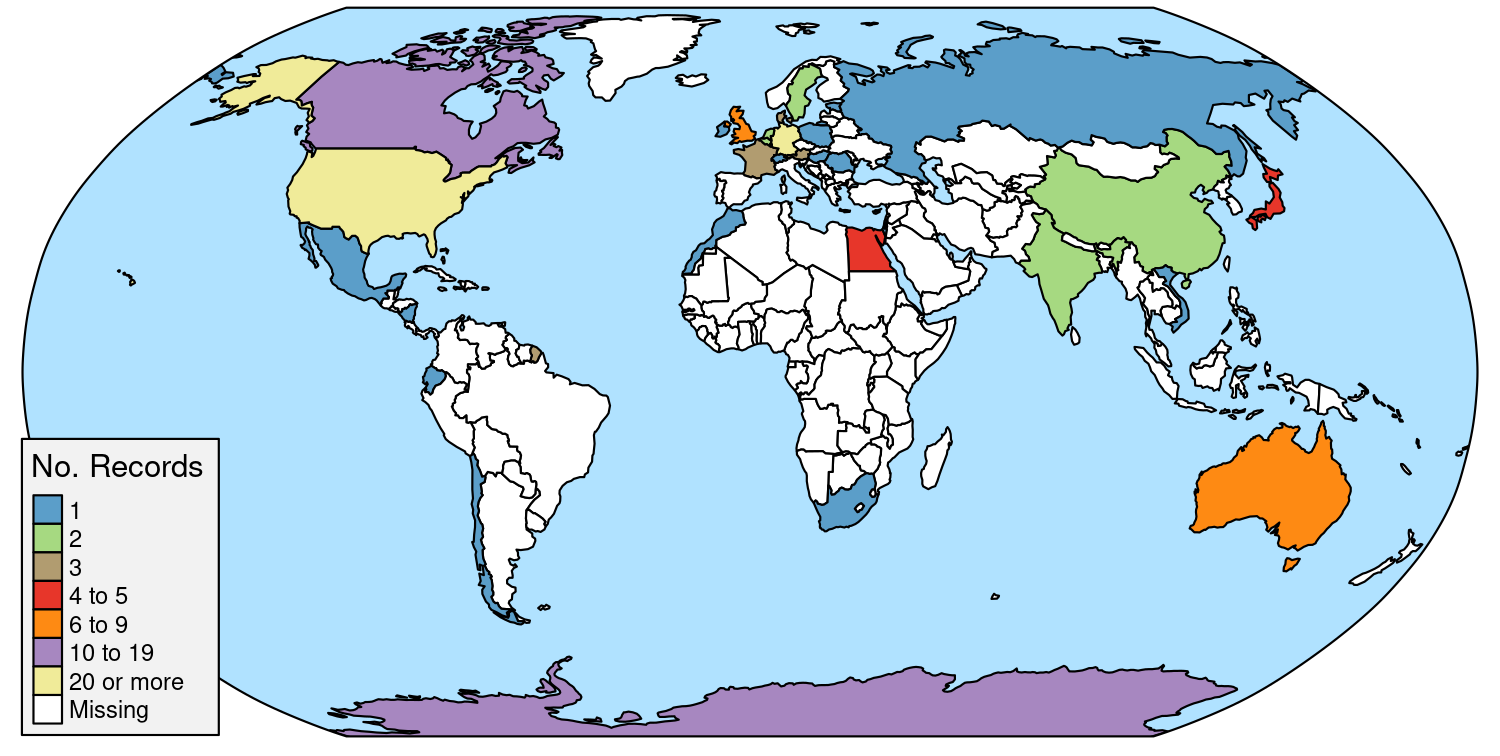
\includegraphics[width=5in,height=2.51944in]{Figures/world_records.png}
\caption{World map showing the distribution of records assigning trophic
resources to soil mesofauna, largely unexplored outside Europe and the
United States.}
\end{figure}

We obtained a total of 3009 records about trophic relationships (ESM
II), with Acari contributing with 2218 records (73,71\%), and within
this number, the majority (50.63\%) correspond to Sarcoptiformes. At the
species level, 168 records were Collembola, and 422 records were Acari.
At the genus level, 572 records were found. The family level adds 210
records with 51 different families out of the total of 161 families
identified in this review.

\hypertarget{methods-used-for-trophic-resources-identification}{%
\subsubsection{Methods used for trophic resources
identification}\label{methods-used-for-trophic-resources-identification}}

\hypertarget{methods-for-resource-assignment}{%
\paragraph{Methods for resource
assignment}\label{methods-for-resource-assignment}}

The method of observations in laboratory tests provides the main
empirical evidence from the database with 706 records (Figure 2).

\begin{figure}
\centering
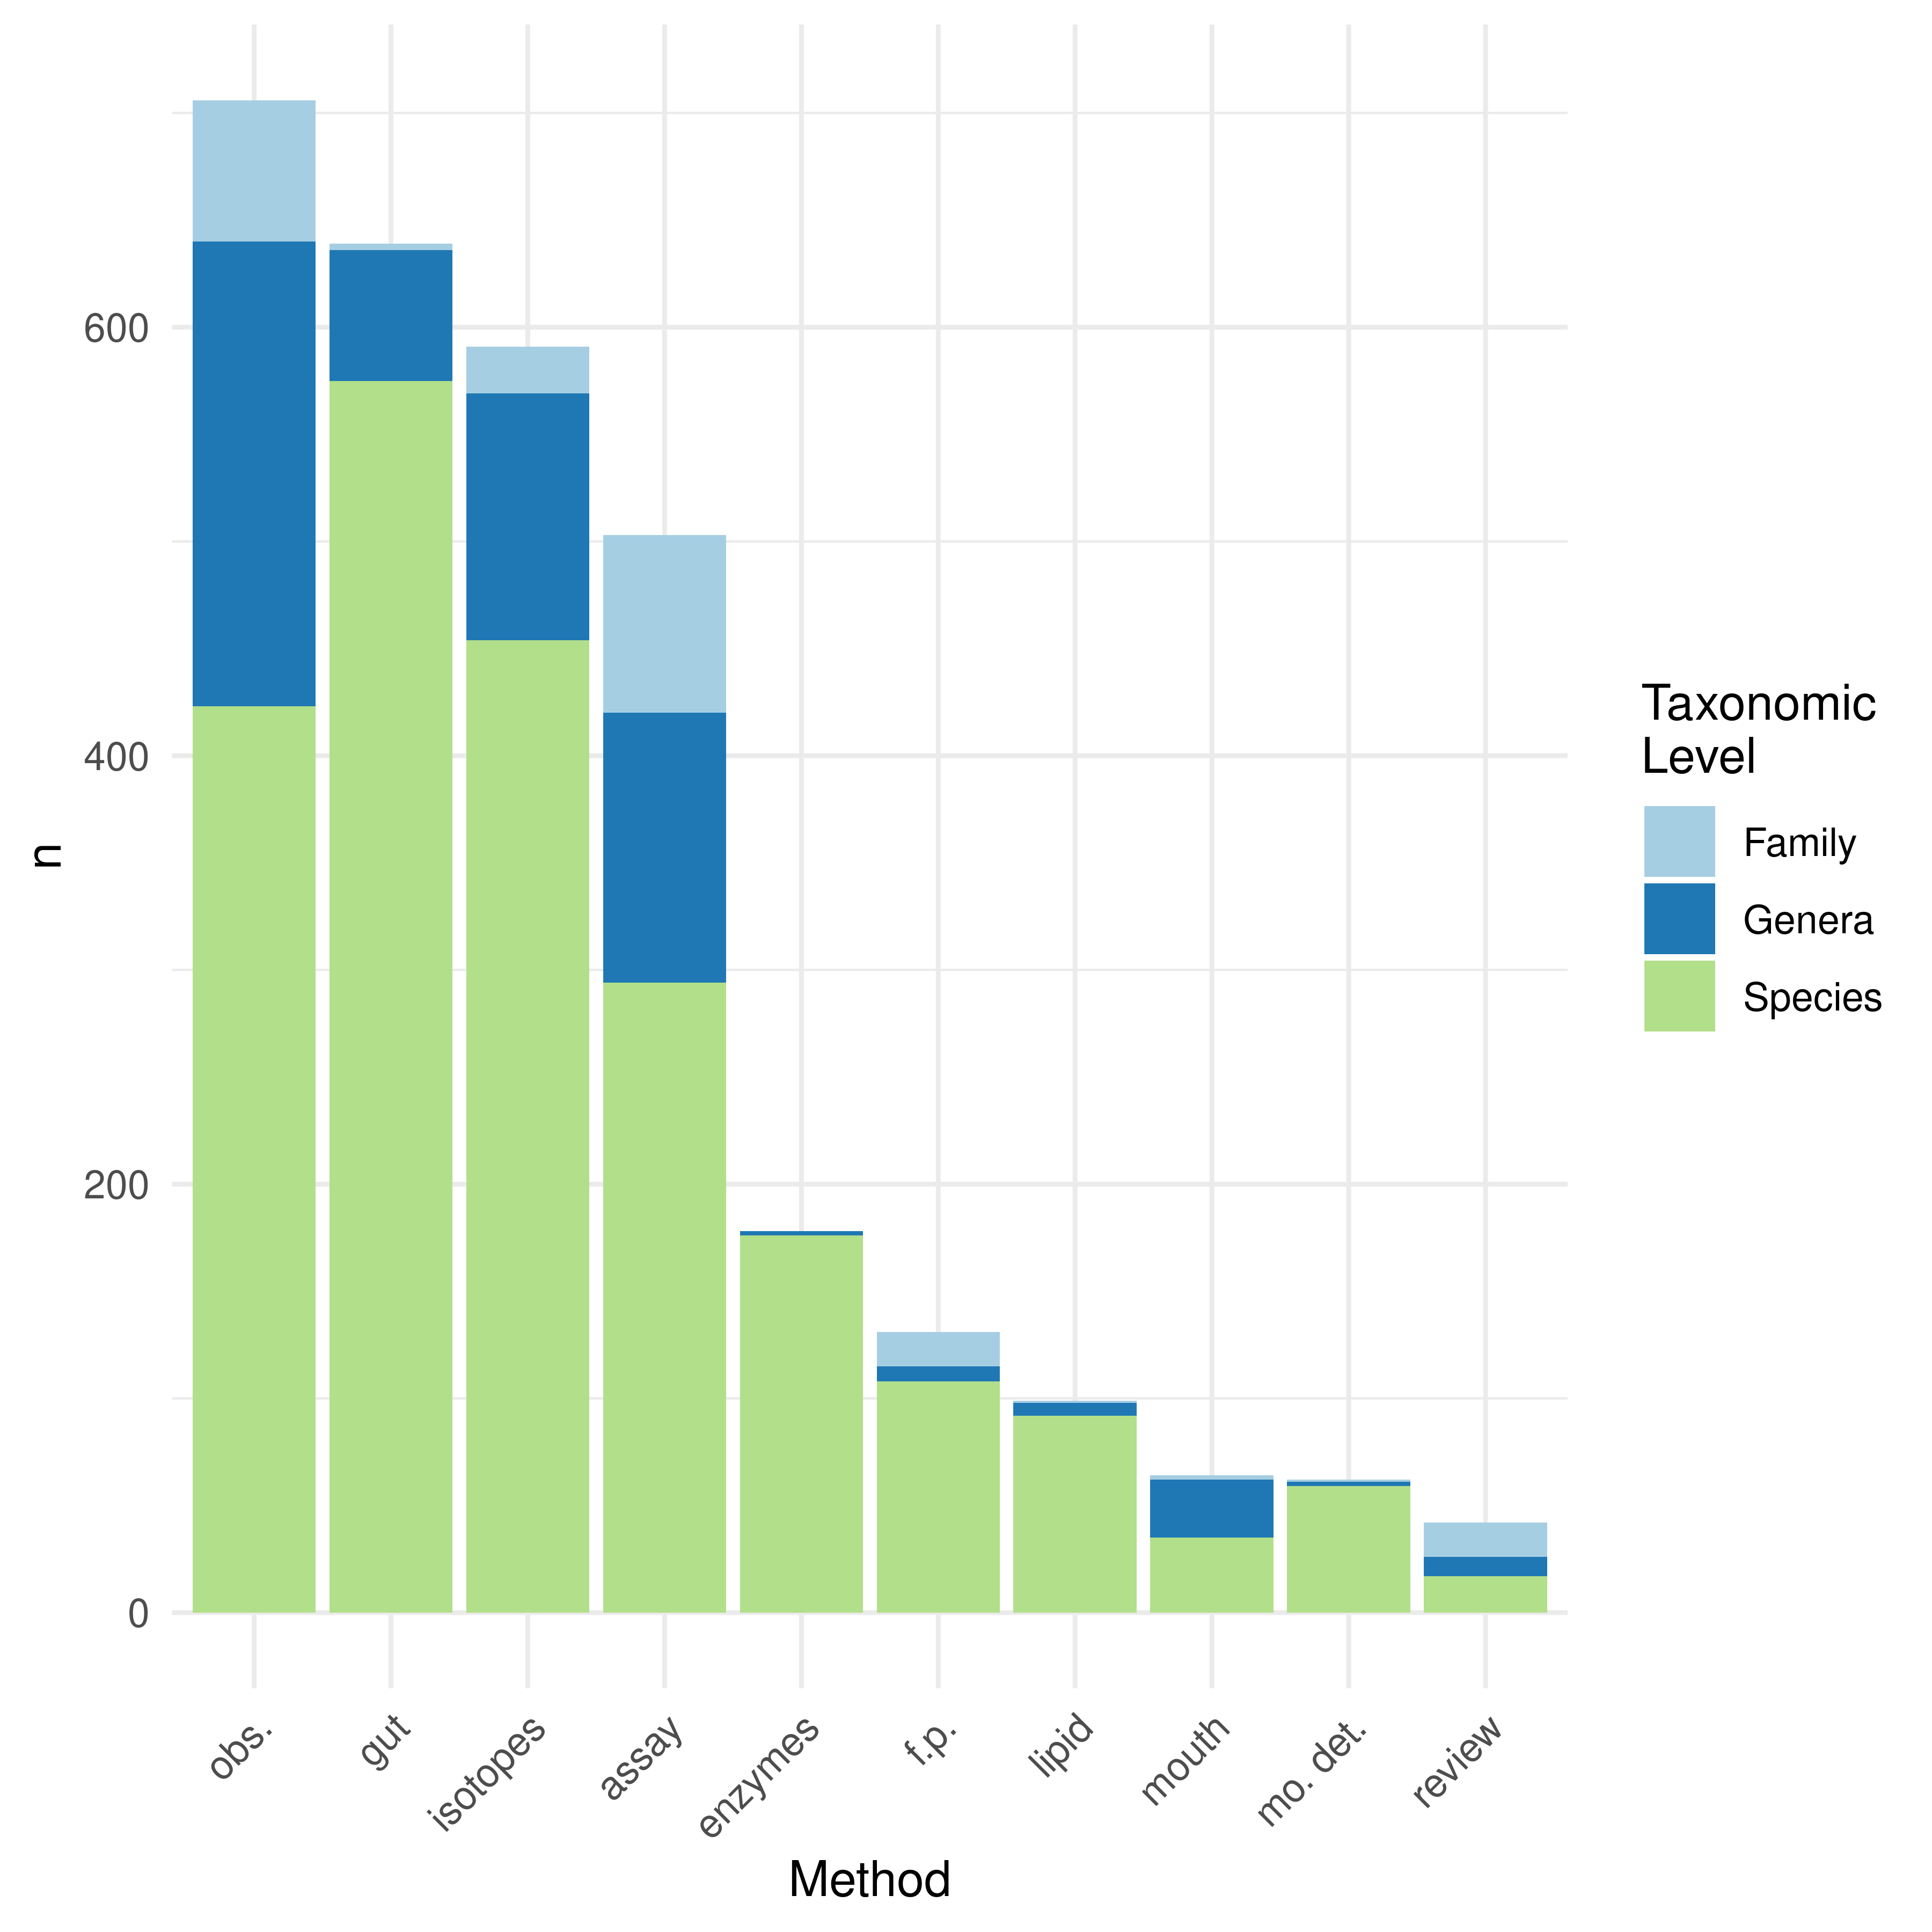
\includegraphics[width=4.92014in,height=4.92014in]{Figures/Metodo_ByTaxLevel.jpeg}
\caption{Methods used in the literature to assign trophic resources to
soil mesofauna taxa. Colors within columns refer to the number of
different taxonomic levels for which each method assigned at least one
resource. Assay: laboratory tests and observations. Isotopes: stable
isotopes. Gut: intestinal content. Enzymes: Digestive enzymes. Mouth:
mouthparts morphology. Lipid: lipid profile. Mo. det: molecular
detection of intestinal content, f.p.: Food preference assays. Obs.:
direct lab observations of feeding activity. Reviews: general reviews by
other authors.}
\end{figure}

Microarthropods at the family level constitute 9.3\% of the observations
in laboratory tests, with 63.6\% of the total corresponding to the
Prostigmata suborder, within which 10 different families are mentioned.
The evidence offered by observations in laboratory tests adds up to
90.7\% for species and genera. The orders Mesostigmata (62.5\%),
Sarcoptiformes (23.8\%), Trombidiformes (9\%) and Arthropleona (4\%) are
the ones with the higher presence in the literature.

The gut content method reaches 21.3\% of the records, in which the
species taxonomic level corresponds to 89.9\% of the total records and
the genus level to 9.5\%.

Stable isotopes follow in importance. From these, 76.9\% of the records
mention species. Genera and family add up to 23.1\% of the records.

The activity of digestive enzymes (178 records) in all cases reports
down to the species level. For this empirical evidence, the authors
worked with the order Sarcoptiforme (Acari) with 38 different species
and Arthropleona and Symphypleona (Collembola) with 17 different
species.

Other three methods accumulate 9.75\% of the records, these being food
preference tests (131 records), the study of fatty acids (99 records),
and the use of mouthpart structures (64 records).

Intestinal contents analyses with molecular techniques for the detection
of DNA is a tool of recent development and represent 0.8\% of the total
records.

\hypertarget{resources-identified-by-empirical-evidence}{%
\paragraph{Resources identified by empirical
evidence}\label{resources-identified-by-empirical-evidence}}

The main resource mentioned corresponds to saprophytic fungi (19.7\%)
followed by microfauna (15.6\%), bacteria (10.8\%), and litter (10.3\%),
the records for mites, collembola, enchytraeidae, larvae, and eggs
accumulate 725 mentions (24\%) (Table 1). It is worth noting that a
higher number of records have been taken to the species level. For
instance, 592 trophic records are associated with saprophytic fungi
consumption, of which 16 were associated with the taxonomic level of the
family, 105 to the genus level, and 471 to the species level.

\begin{figure}
\centering
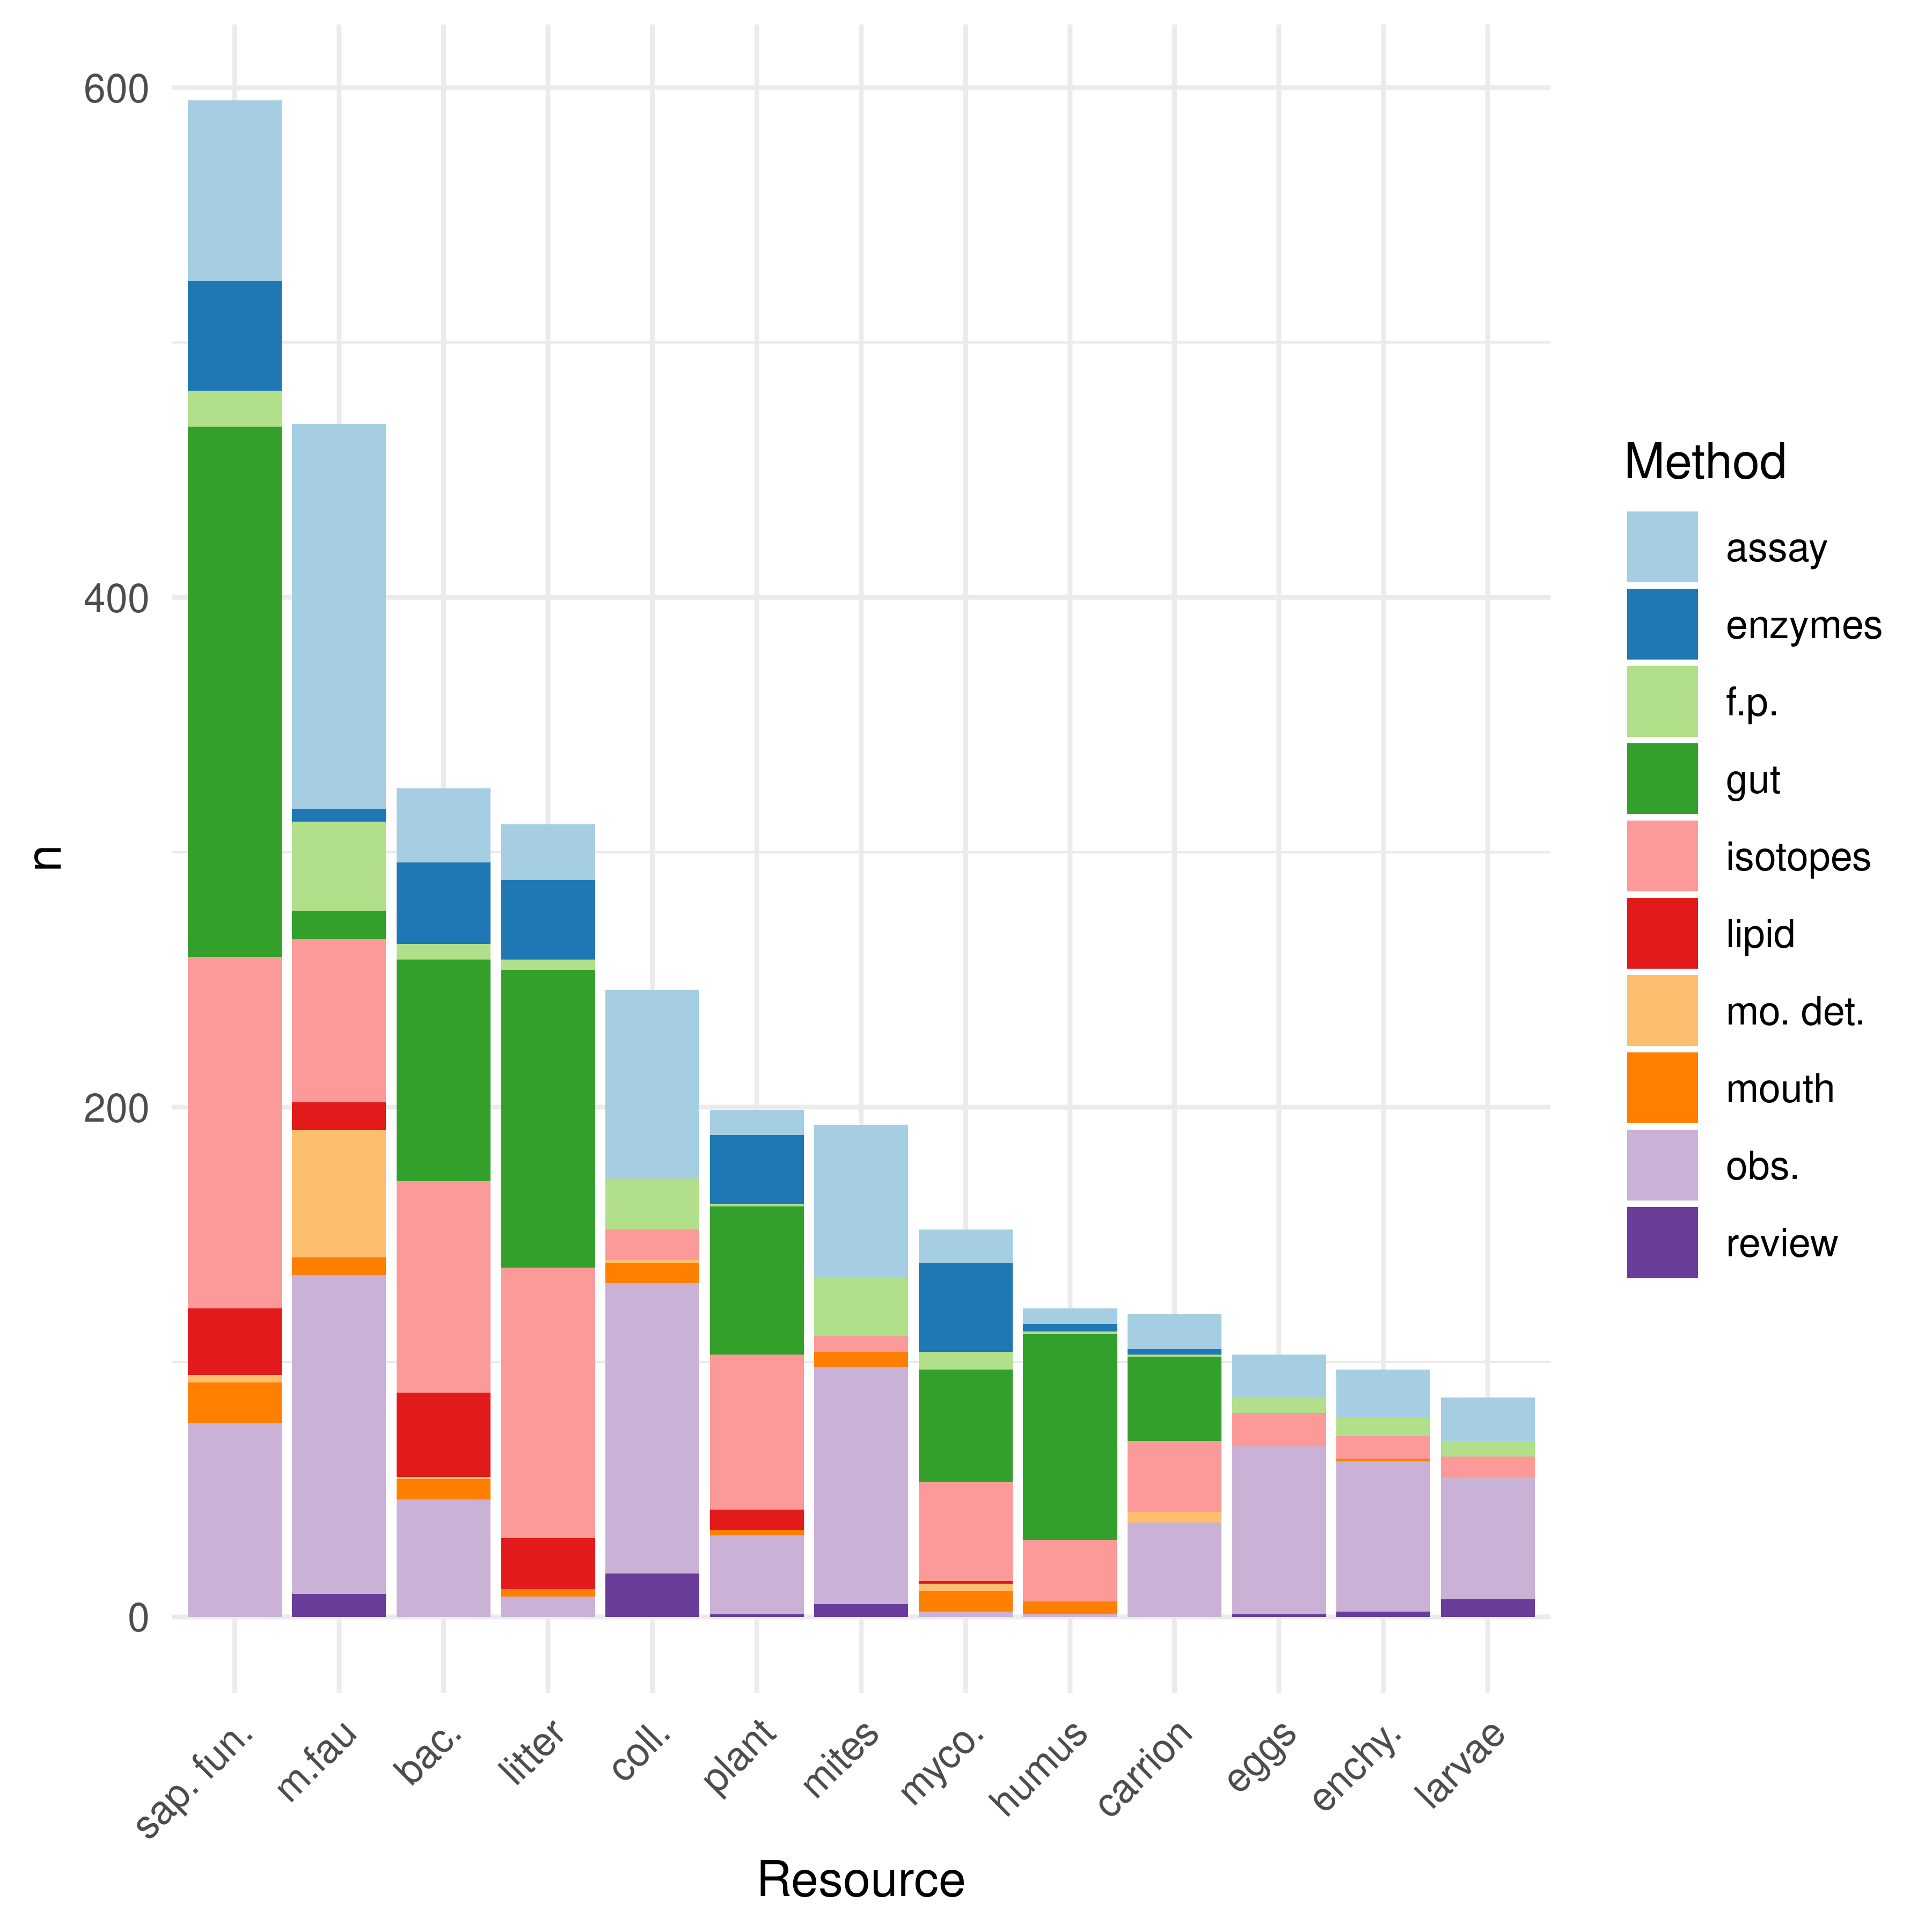
\includegraphics[width=5.11667in,height=5.11667in]{Figures/Recursos_ByMetodo.jpeg}
\caption{The number of records in the literature assigning each one of
the 13 trophic resources to a mesofauna taxon as shown in Table 1.
Colors in the columns refer to the method used to assign those trophic
resources to a particular taxon. Methods as in Fig. 2.}
\end{figure}

Laboratory observations (the most used method), mention the use of the
thirteen trophic resources (Figure 3) in which the order of importance
according to the number of mentions is microfauna \textgreater{}
springtails \textgreater{} mites \textgreater{} saprophytic fungi
\textgreater{} invertebrate eggs \textgreater{} enchytraeids
\textgreater{} larvae of invertebrates that accumulate 82.3\%. For this
empirical method, the main resources correspond to typical resources of
predatory animals except for saprophytic fungi, the main taxa mentioned
is Mesostigmata. Figure 3 also shows (in colors) that the most important
methods used for resource assignment, according to the number of
citations in the bibliography, was: direct observations (706 records)
\textgreater{} gut contents (639) \textgreater{} isotopes (591)
\textgreater{} lab assays (503) \textgreater{} enzymes (178)
\textgreater{} feeding preference assays (131 records).

The methodologies that use laboratory studies, i.e.~laboratory tests,
laboratory observations, and food preference tests, provide direct
evidence of the use of the trophic resources, constituting together
44.5\% of the empirical evidence analyzed. (ESM II) These laboratory
methods are the ones that most frequently mention the use of animal
resources, springtails - mites - invertebrate larvae - invertebrate eggs
- enchytraeids, as food resources. These methods rarely mention the
consumption of Mycorrhizal fungi and rarely the use of humus.

\hypertarget{use-of-trophic-resources-by-soil-microarthropods}{%
\subsubsection{Use of trophic resources by soil
microarthropods}\label{use-of-trophic-resources-by-soil-microarthropods}}

It is interesting to note that at the family level, the most numerous
records correspond to trophic resources such as springtail, mites,
microfauna, larvae, invertebrate eggs, and enchytraeids, typical
resources of predatory microarthropods (Table 2). Similarly, at the
genus level, the typical resources of predators represent 54\% of the
records. At the species level, the main resource mentioned is
saprophytic fungi.

The use of trophic resources in the six main orders mentioned in the
literature (3 orders of Collembola and 3 orders of Acari) are divided
into their families, genera, and species in a nested way (Table 2). For
example, for the order Symphypleona (Sy), the empirical evidence studies
13 species included in 10 genera within 3 families. In this way, Table 2
shows also for Symphypleona (Sy), that 8 of the 13 species mentioned,
within 7 of the 10 genera, within 2 of the 3 families in the available
bibliography, are mentioned consuming Saprophytic fungi. For additional
identity and information on families, genera and species see ESM II.

In all the taxonomic hierarchies considered, the order Sarcoptiformes
(Acari) consumes mainly saprophytic fungi, bacteria, litter, plant
tissues, and Mycorrhizal fungi. The order Trombidiformes (Acari), are
presented mainly as predators.

For Collembola, the diversity of species addressed by empirical evidence
is grouped into only 13 families, 3 of which belong to Symphypleona and
a family of Neelipleona.

The empirical evidence that addresses the trophic study of Arthropleona
(Collembola) is represented by 154 different species, these were mainly
associated with saprophytic fungi (119 species), followed in importance
by bacteria, litter and humus. The microfauna is mentioned as a resource
for 39 species.

\begin{figure}
\centering
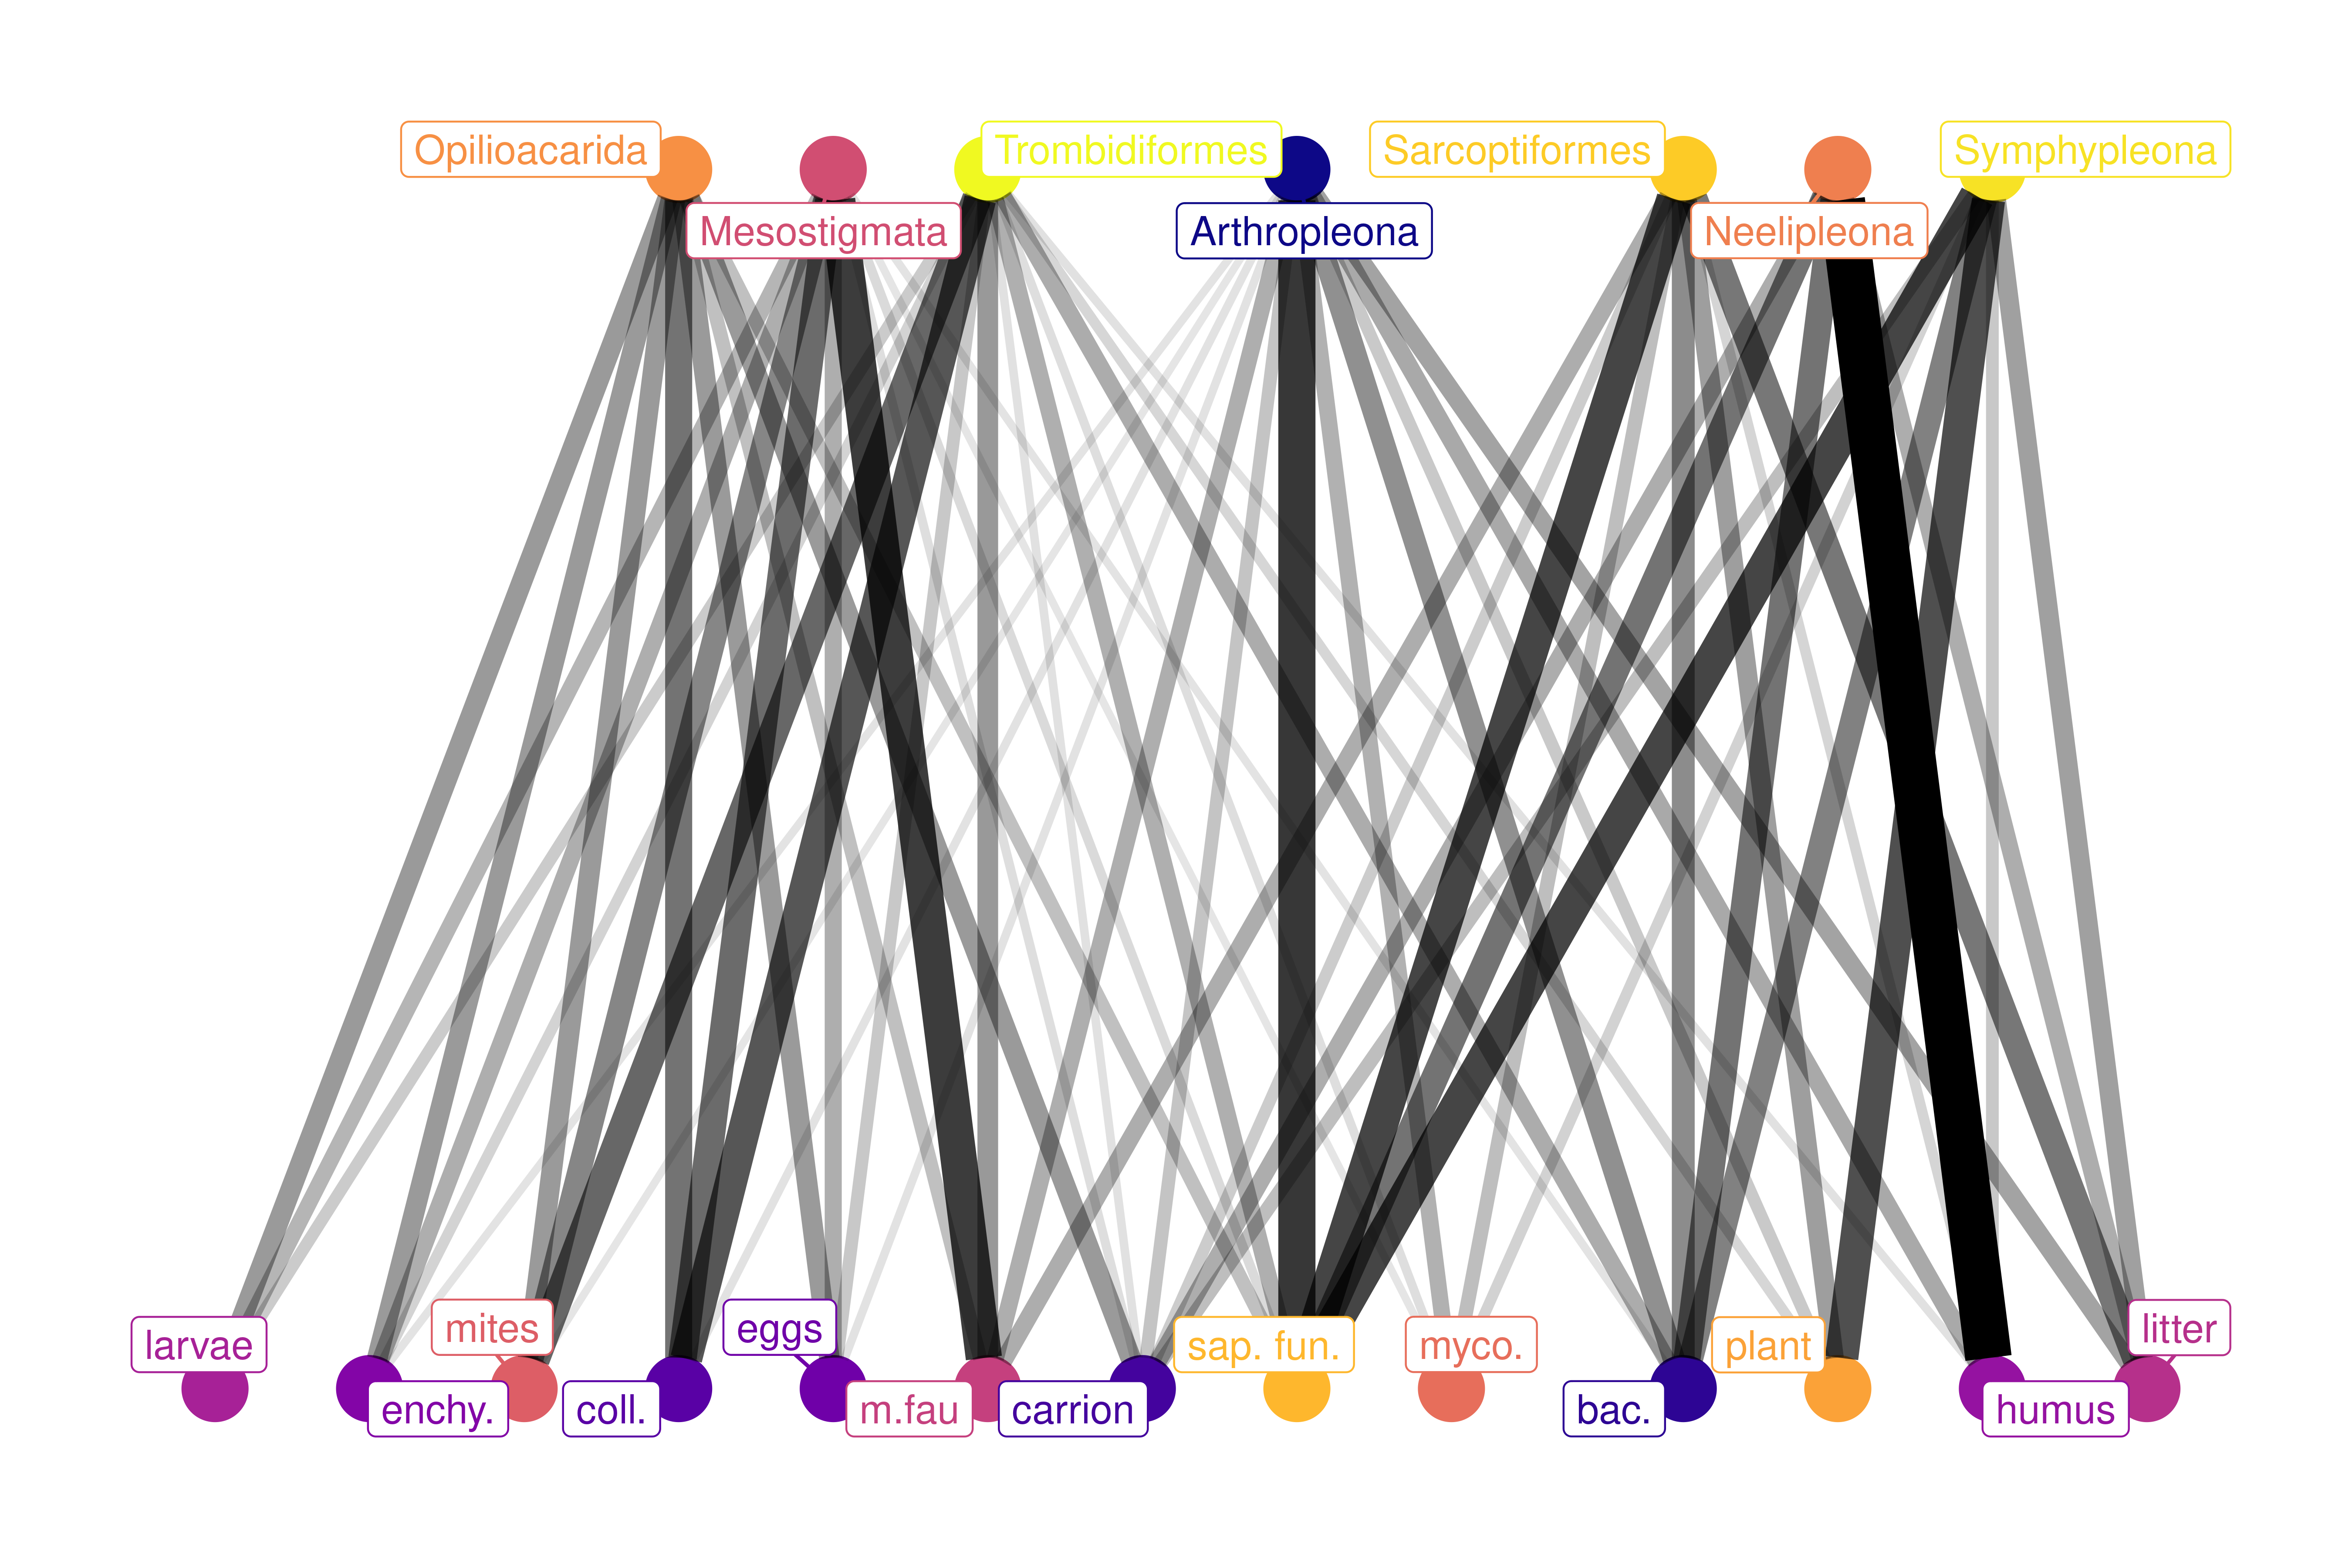
\includegraphics[width=5.4125in,height=3.60833in]{Figures/Bi_Orden_Recurso.jpeg}
\caption{Bipartite graph showing the use of trophic resources by the
main orders of Acari and Collembola. Upper nodes: Acari and Collembola
orders as in Table 2. Lower nodes: trophic resources. The thickness and
intensity of the lines give an idea of the proportion of mentions in the
available literature about their use of trophic resources. Resource
names as in Tables 1 and 2.}
\end{figure}

Figure 4 presents the proportion of resources used by the main 3 mite
orders and 3 Collembola orders, as found in the literature. For
instance, the resource of saprophytic fungi is the main constituent of
the diet of the Arthropleona, being the bacteria, the litter, the humus,
and the microfauna mentioned resources in lesser proportion.
Trombidiformes have a diet based mainly on microarthropods and nematodes
and to a lesser extent saprophytic fungi and bacteria.

\hypertarget{discussion}{%
\subsection{Discussion}\label{discussion}}

Until the 1960s, soil fauna was considered mainly earthworms, and
terrestrial ecologists considered most of the soil fauna as a ``black
box'' of decomposers and detritivores (Briones, 2014). The information
gradually collected over the following decades regarding the edaphic
microarthropods is reaching the point where it is possible to focus on
integrative works. (Pautasso 2013) However, the available information is
still scarce and mostly restricted to the most numerous or conspicuous
groups of the soil microarthropods, mainly from European soils.

For soil microarthropods, the evidence provided by laboratory work
results in the most straightforward traditional method to know how these
animals use trophic resources, their feeding behavior, their food
preferences, and their development and growth in controlled
environments, but Feeding links observed in the laboratory do not
necessarily relevant for the field (Nielsen 2018, Potapov 2022). The
method used to relate the isotopic signature of organisms and their
resources is a recently developed tool that is useful for detecting the
importance and the changes in time or space of assumed trophic
relationships, which means that we have to know in advance if the
trophic relationship exists. The main drawback of the method is that if
we erroneously assign a trophic relationship the proportions of the
diets could be greatly distorted from the real trophic relationships. On
the other side, this method has several advantages 1) it can analyze a
large number of species and an important variety of resources (Potapov
et al., 2019), 2) it can provide field evidence of real interactions

3) it can provide quantitative data, accounting for interaction strength

4) it can provide information on assimilation and not only ingestion
(Nielsen et al.~2018)

The different methods have different sources of errors so it will be
desirable that trophic resources used by soil microarthropods can be
determined in a complementary way with several methods (Potapov et al.,
2020; Walter et al.,1991).

The most used resources are saprophytic fungi, microfauna, and bacteria.
If we associate them with their nutritional characteristics, these
trophic resources are rich in molecules with great nutritional value as
determined in the dietary routes labeled by fatty acids, stable
isotopes, or the enzymatic methods (Nielsen, 1962; Potapov et al., 2019;
Ruess and Chamberlain, 2010).

It is also to be noted that the information available for Acari and
Collembola is strongly asymmetric, corresponding mainly to Acari, order
Sarcoptiformes.

Despite the increasing amount of descriptive works and lists of
taxonomic groups, the information available worldwide is still largely
fragmentary and incomplete, and taxonomic resolution varies considerably
between and within published works.

We found that a large proportion of the resources are defined as
taxonomic categories of species, genera, and families, which would be
important to estimate the diets of higher taxonomic groups. The
available information for low taxonomic levels could be used as a
reference to address the problem of what the use of soil resources will
be like by higher-level taxonomic groups (Bedano, 2007; Potapov et
al.~2020).

This information must be interpreted with caution, however, because
within a taxonomic category, each species could apply different
strategies to the problem of exploiting resources (Lavelle and Spain,
2001; Moore et al.,1988), as many taxa in the available literature are
considered to be general consumers.

The results presented here provide valuable new information about the
different feeding strategies of the main groups of the soil
microarthropods, and also on the quality and usefulness of the different
methods used to assign trophic resource use to different taxa. It also
presents the current status of knowledge about soil microarthropods
trophic resources usage. Moreover, it highlights the still quite scant
information available in this regard.

Finally, it is necessary to call attention to the need for more studies
on the trophic relationships of the soil microarthropods. Out of a total
of approximately 9000 described species of Collembola (Bellinger et al.,
2020), it was only possible to find trophic information for just 127
soil inhabitant species. For Acari, out of the approximately 58,000
species described (Schmidt, 2020), it was only possible to find
references of trophic relationships for 307 soil species.

It is clear that big gaps in the available information must be filled to
advance our knowledge on the structure and functioning of soil food
webs. Not only are there several microarthropods groups hardly explored,
but also the geographical coverage is still quite narrow. Almost 52\% of
the published studies about the trophic resources of Acari and
Collembola were developed in European countries. Further deepening on
the knowledge of functional and trophic relationships of the soil the
fauna would allow for a better and more precise evaluation of the
functioning of the edaphic ecosystem, the protection of the ecosystem
services that the soil microarthropods provide, and the sustainable use
of the soil.

\hypertarget{acknowledgements}{%
\subsection{Acknowledgements}\label{acknowledgements}}

The authors wish to thank the help of Dr.~Fernando Momo for his useful
comments to previous versions of this work. To Dr.~Mark Breidenbaugh for
his help in reviewing the English language usage and grammar.

\hypertarget{declarations}{%
\subsection{Declarations}\label{declarations}}

This work was partially funded by a scholarship to Victor N. Velazco
from Consejo Nacional de Ciencia y Tecnología (CONICET). This research
did not receive any other specific grant from funding agencies in the
public, commercial, or not-for-profit sectors. The authors declare no
conflicts of interest. All the data for this work not shown here are
available as Electronic Supplementary Material and referred to in the
text when appropriate.

\textbf{Conflict of Interest:} The authors declare they have no conflict
of interest.

\hypertarget{bibliography}{%
\subsection{Bibliography}\label{bibliography}}

Anderson JM., 1978. A method to quantify soil-microhabitat complexity
and its application to a study of soil animal species diversity. Soil
Biol. Biochem. 10, 77--78. https://doi.org/10.1016/0038-0717(78)90014-7

Anderson JM., 1977. The Organization of Soil Animal Communities. Ecol.
Bull. 25, 15--23.

Barrios E., 2007. Soil biota, ecosystem services, and land productivity.
Ecol. Econ. 64, 269--285. https://doi.org/10.1016/j.ecolecon.2007.03.004

Bedano JC., 2007.El rol de la mesofauna edáfica en la evaluación de la
calidad del Suelo, In: De La Biología de Los Suelos a La Agricultura.
Universidad Nacional de Río Cuarto. pp.~247--258.

Behan-Pelletier V, Newton G., 1999. Linking soil biodiversity and
ecosystem function. The taxonomic dilemma. BioScience 2.
\href{https://doi.org/10.2307/1313540}{\underline{https://doi.org/10.2307/1313540}}.

Bellinger PF, Christiansen KA, Janssens F., 2020. Internet resource
available from:
\href{http://www.collembola.org/}{\underline{http://www.collembola.org}}.
Last updated: November 30, 2020. Last accessed: December 23, 2020.

Berg, M.P., Stoffer, M., van den Heuvel, H. 2004. Feeding guilds in
Collembola based on digestive enzymes. Pedobiologia 48, 589-601. DOI:
\href{http://dx.doi.org/10.1016\%2Fj.pedobi.2004.07.006}{\underline{\hfill\break
10.1016/j.pedobi.2004.07.006}}

Berg B, McClaugherty C., 2008. Plant litter: decomposition, humus
formation, carbon sequestration, 2nd. ed.~Springer, Berlin.

Briand F, Cohen JE., 1984 Community food webs have scale-invariant
structure. Nature, Letters to Nature. 307, 264--267.

Briones MJI., 2014. Soil fauna and soil functions: a jigsaw puzzle.
Front. Environ. Sci. 2, 1--22. https://doi.org/10.3389/fenvs.2014.00007

Brussaard L., 1977. Biodiversity and Ecosystem Functioning in Soil.
Ambio. 26, 563--570.

Buryn R, Brandl R., 1992. Are the morphometrics of chelicerae correlated
with diet in mesostigmatid mites (Acari)? Exp. Appl. Acarol. 14, 67--82.
\href{https://doi.org/10.1007/BF01205353}{\underline{https://doi.org/10.1007/BF01205353}}

Chamberlain, P. M., Bull, I. D., Black, H. I. J., Ineson, P., \&
Evershed, R. P. (2006). Collembolan trophic preferences determined using
fatty acid distributions and compound-specific stable carbon isotope
values. Soil Biology and Biochemistry, 38(6), 1275-1281.

Chernova NM, Bokova AI, Varshav EV, Goloshchapova NP, Savenkova YuYu.,
2007. Zoophagy in Collembola. Entomol. Rev.~87, 799--811.
https://doi.org/10.1134/S0013873807070020

Clark FE., 1971. Bacterios del Suelo, In: Burges, A., Raw, F. (Eds.),
Biología del Suelo, Chapter 2. Ediciones Omega, Barcelona. pp.~27--68.

Cragg RG, Bardgett RD., 2001. How changes in soil faunal diversity and
composition within a trophic group influence decomposition processes.
Soil Biol. Biochem. 33, 2073--2081.
https://doi.org/10.1016/S0038-0717(01)00138-9

FAO, ITPS, GSBI, SCBD, EC., 2020. State of knowledge of soil
biodiversity. Status, challenges and potentialities, Report 2020; Rome,
FAO. https://doi.org/10.4060/cb1928en

Hartenstein R., 1962. Soil Oribatei. I. Feeding Specificity among Forest
Soil Oribatei (Acarina). Ann. Entomol. Soc. Am. 55, 202--206.
https://doi.org/10.1093/aesa/55.2.202

Hättenschwiler S, Tiunov AV, Scheu, S., 2005. Biodiversity and Litter
Decomposition in Terrestrial Ecosystems. Annu. Rev.~Ecol. Evol. Syst.
36, 191--218. https://doi.org/10.1146/annurev.ecolsys.36.112904.151932

Heidemann K, Ruess L, Scheu S, Maraun M., 2014. Nematode consumption by
mite communities varies in different forest microhabitats as indicated
by molecular gut content analysis. Exp. Appl. Acarol. 64, 49--60.
https://doi.org/10.1007/s10493-014-9807-x

Hooper DU, Chapin FS, Ewel JJ, Hector A, Inchausti P, Lavorel S, Lawton
JH, Lodge DM, Loreau M, Naeem S, Schmid B, La HS, Symstad AJ, Vandermeer
J, Wardle DA., 2005. Effects of biodiversity on ecosystem functioning: A
consensus of current knowledge. Ecol. Monogr. 75, 33.
\href{https://doi.org/10.1890/04-0922}{\underline{https://doi.org/10.1890/04-0922}}

Hopkin, S. P. (1997).~Biology of the springtails: (Insecta: Collembola).
Oxford University Press. Oxford, UK. 340 pp.

Hubert J, Žilová M, Pekár, S., 2001. Feeding preferences and gut
contents of three panphytophagous oribatid mites (Acari: Oribatida).
Eur. J. Soil Biol. 37, 197--208.
https://doi.org/10.1016/S1164-5563(01)01083-4

International Commission on Zoological Nomenclature. Internet resource.
iczn.org, last accessed: September 13, 2021.

IPBES, 2019. Global assessment report on biodiversity and ecosystem
services of the Intergovernmental Science-Policy Platform on
Biodiversity and Ecosystem Services. Brondizio ES, Settele J, Díaz S,
Ngo HT (eds). IPBES secretariat, Bonn, Germany.

Kaneko N., 1988. Feeding habits and cheliceral size of oribatid mites in
cool temperate forest soils in Japan. Rev.~Écologie Biol. Sol. 25,
353--363.

King RA, Read DS, Traugott M, Symondson WOC., 2008. Molecular analysis
of predation: A review of best practice for DNA-based approaches. Mol.
Ecol. 17, 947--963. https://doi.org/10.1111/j.1365-294X.2007.03613.x

Krantz GW, Walter DE (Eds.), 2009. A manual of acarology, 3rd ed. Texas
Tech University Press, Lubbock, Texas.

Kühn J, Schweitzer K, Ruess L., 2019. Diversity and specificity of lipid
patterns in basal soil food web resources. PLOS ONE 14, e0221102.
https://doi.org/10.1371/journal.pone.0221102

Lavelle P., 1996. Diversity of soil fauna and ecosystem function. Biol.
International 33, 3--16.

Lavelle P, Decaëns T, Aubert M, Barot S, Blouin M, Bureau F, Margerie P,
Mora P, Rossi JP., 2006. Soil invertebrates and ecosystem services. Eur.
J. Soil Biol. 2006; 42, S3--S15.
https://doi.org/10.1016/j.ejsobi.2006.10.002

Lavelle P, Spain AV., 2001. Soil Ecology, 2nd. ed.~Kluwer Academic
Publisher. Springer.

Martínez PA, Narciso EN., 2009. Mesofauna. In: Momo, F.R., Falco, L.B.
(Eds.), Biología y Ecología de la Fauna del Suelo. Imago Mundi, Buenos
Aires, p.~186.

Martín-López, B, González JA, Díaz S, Castro I, García-Llorente M.,
2007. Biodiversidad y bienestar humano: el papel de la diversidad
funcional. Ecosistemas. 16, 69--80.

Moore JC, Walter, DE, Hunt, HW., 1988. Arthropod Regulation of Micro-
and Mesobiota in Below-Ground Detrital Food Webs. Annu. Rev.~Entomol.
33, 419--435. https://doi.org/10.1146/annurev.en.33.010188.002223

Nielsen CO., 1962. Carbohydrases in Soil and Litter Invertebrates.
Oikos. 13, 200--2015. https://doi.org/10.2307/3565085

Nielsen JM, Clare EL, Hayden B, Brett MT, Kratina P., 2018. Diet tracing
in ecology: Method comparison and selection. Methods Ecol. Evol. 9,
278--291. https://doi.org/10.1111/2041-210X.12869

Nielsen UN, Osler GHR, Campbell CD, Neilson R, Burslem DFRP, van der Wal
R., 2010. The Enigma of Soil Animal Species Diversity Revisited: The
Role of Small-Scale Heterogeneity. PLoS ONE. 5, e11567.
https://doi.org/10.1371/journal.pone.0011567

Pankhurst C., Doube BM, Gupta VVSR., 1997. Biological Indicators of Soil
Health. CAB INTERNATIONAL.

Persson T, Bååth E, Clarholm M, Lundkvist H, Söderström BE, Sohlenius
B., 1980. Trophic Structure, Biomass Dynamics and Carbon Metabolism of
Soil Organisms in a Scots Pine Forest. Ecol. Bull. 32, 419--459.

Petersen H, Luxton, MA., 1982. Comparative Analysis of Soil Fauna
Populations and Their Role in Decomposition Processes. Oikos. 39, 288.
https://doi.org/10.2307/3544689

Pey B, Nahmani J, Auclerc A, Capowiez Y, Cluzeau D, Cortet J, Decaëns T,
Deharveng L, Dubs F, Joimel S, Briard C, Grumiaux F, Laporte MA, Pasquet
A, Pelosi C, Pernin C, Ponge JF, Salmon S, Santorufo L, Hedde M., 2014.
Current use of and future needs for soil invertebrate functional traits
in community ecology. Basic Appl. Ecol. 15, 194--206.
\href{https://doi.org/10.1016/j.baae.2014.03.007}{\underline{https://doi.org/10.1016/j.baae.2014.03.007}}.

Pautasso, M. (2013). Ten simple rules for writing a literature review.
\emph{PLoS computational biology}, \emph{9}(7), e1003149.

Pollierer MM, Scheu S, Haubert D., 2010. Taking it to the next level:
Trophic transfer of marker fatty acids from basal resource to predators.
Soil Biol. Biochem. 42, 919--925.
\href{https://doi.org/10.1016/j.soilbio.2010.02.008}{\underline{https://doi.org/10.1016/j.soilbio.2010.02.008}}

Pollierer, M. M., \& Scheu, S. (2021). Stable isotopes of amino acids
indicate that soil decomposer microarthropods predominantly feed on
saprotrophic fungi. \emph{Ecosphere}, \emph{12}(3), e03425.

Pollierer, M. M., Larsen, T., Potapov, A., Brückner, A., Heethoff, M.,
Dyckmans, J., \& Scheu, S. (2019). Compound specific isotope analysis of
amino acids as a new tool to uncover trophic chains in soil food webs.
Ecological Monographs, 89(4), e01384.

Ponge JF., 1991. Food resources and diets of soil animals in a small
area of Scots pine litter. Geoderma. 49, 33--62.
https://doi.org/10.1016/0016-7061(91)90090-G

Potapov AM, Pollierer MM, Salmon S, Šustr V, Chen TW., 2020.
Multidimensional trophic niche approach: gut content, digestive enzymes,
fatty acids, and stable isotopes in Collembola. bioRxiv
2020.05.15.098228.
\href{https://doi.org/10.1101/2020.05.15.098228}{\underline{https://doi.org/10.1101/2020.05.15.098228}}

Potapov AM, Tiunov AV, Scheu S., 2019. Uncovering trophic positions and
food resources of soil animals using bulk natural stable isotope
composition: Stable isotopes in soil food web studies. Biol. Rev.~94,
37--59. \underline{https://doi.org/10.1111/brv.12434}

R Core Team (2021). R: A language and environment for statistical
computing. R Foundation for Statistical Computing, Vienna, Austria.
https://www.R-project.org/.

Read DS, Sheppard SK, Bruford MW, Glen DM, Symondson WOC., 2006.
Molecular detection of predation by soil micro-arthropods on nematodes.
Mol. Ecol. 15, 1963--1972.
https://doi.org/10.1111/j.1365-294X.2006.02901.x

Ruess L, Chamberlain PM., 2010. The fat that matters: Soil food web
analysis using fatty acids and their carbon stable isotope signature.
Soil Biol. Biochem. 42, 1898--1910.
https://doi.org/10.1016/j.soilbio.2010.07.020

Ruess L, Schütz K, Migge-Kleian S, Häggblom MM, Kandeler E, Scheu S.,
2007. Lipid composition of Collembola and their food resources in
deciduous forest stands---Implications for feeding strategies. Soil
Biol. Biochem. 39, 1990--2000.
https://doi.org/10.1016/j.soilbio.2007.03.002

Rusek J., 1998. Biodiversity of Collembola and their functional role in
the ecosystem. Biodivers. Conserv. 7, 1207--1219.
https://doi.org/10.1023/A:1008887817883

Saur É, Ponge J., 1988. Alimentary studies on the Collembolan
Paratullbergia callipygos using transmission electron microscopy.
Pedobiologia. 31, 355--379.

Schmidt KH., 2020. Internet resource available from:
\href{http://miteresearch.org/}{\underline{http://miteresearch.org}}.
Last accessed: December 23, 2020.

Schneider K., 2005. Feeding biology and diversity of oribatid mites
(Oribatida, Acari). PhD dissertation. Technischen Universität Darmstadt.
Available from:
https://tuprints.ulb.tu-darmstadt.de/585/1/Dissertation\_Schneider.pdf.

Schneider K, Maraun M., 2009. Top-down control of soil microarthropods -
Evidence from a laboratory experiment. Soil Biol. Biochem. 41, 170--175.
https://doi.org/10.1016/j.soilbio.2008.10.013

Schneider K, Renker C, Maraun M., 2005. Oribatid mite (Acari, Oribatida)
feeding on ectomycorrhizal fungi. Mycorrhiza. 16, 67--72.
https://doi.org/10.1007/s00572-005-0015-8.

Schneider K, Renker C, Scheu S, Maraun M., 2004. Feeding biology of
oribatid mites: a minireview. Phytophaga. 14, 247--256.

Siepel H, Ruiter-Dijkman EM., 1993. Feeding guilds of oribatid mites
based on their carbohydrase activities. Soil Biol. Biochem. 25,
1491--1497. https://doi.org/10.1016/0038-0717(93)90004-U.

Thakur MP, Phillips HRP, Brose U, De Vries FT, Lavelle P, Loreau M,
Mathieu J, Mulder C, Van der Putten WH, Rillig MC, Wardle DA, Bach EM,
Bartz MLC, Bennett JM, Briones MJI, Brown G, Decaëns T, Eisenhauer N,
Ferlian O, Guerra CA, König‐Ries B, Orgiazzi A, Ramirez KS, Russell DJ,
Rutgers M, Wall DH, Cameron EK., 2020. Towards an integrative
understanding of soil biodiversity. Biol. Rev.~95, 350--364.
https://doi.org/10.1111/brv.12567

Thompson RM, Brose U, Dunne JA, Hall RO Jr, Hladyz S, Kitching RL,
Martinez ND, Rantala H, Romanuk TN, Stoufer DB, Tylianakis JM., 2012.
Food webs: reconciling the structure and function of biodiversity.
Trends Ecol. Evol. 27, 689--697.
http://dx.doi.org/10.1016/j.tree.2012.08.005

Tiunov AV., 2007. Stable isotopes of carbon and nitrogen in soil
ecological studies. Biol. Bull. 34, 395--407.
https://doi.org/10.1134/S1062359007040127.

van Straalen NM., 1998. Community structure of soil arthropods as a
Bioindicator of Soil Health, in Pankhurst, C., Doube, B.M., Gupta,
V.V.S.R. (Eds.), Biological Indicators of Soil Health. CAB
INTERNATIONAL, U.K. 1998; pp.~235--264.

Walker BH., 1992. Biodiversity and ecological redundancy. Conserv. Biol.
6, 18--23. https://doi.org/10.1046/j.1523-1739.1992.610018.x

Wall DH, Bardgett RD, Behan-Pelletier V, Herryck JE, Jones HT, Ritz K,
Six J, Strong DR, Van der Putten WH., 2012. Soil ecology and ecosystem
services, Journal of Chemical Information and Modeling. Oxford
University Press.

Wall DH, Moore JC., 1999. Interactions underground. Soil biodiversity,
mutualism, and ecosystem processes. BioScience. 49, 109--117.
https://doi.org/10.2307/1313536

Wallwork JA., 1958. Notes on the Feeding Behaviour of Some Forest Soil
Acarina. Oikos. 9, 260--271. https://doi.org/10.2307/3564770

Walter DE, Kaplan DT, Permar TA., 1991. Missing links: a review of
methods used to estimate trophic links in soil food webs. Agric.
Ecosyst. Environ. 34, 399--405.
https://doi.org/10.1016/0167-8809(91)90123-F

Warcup JH., 1971. Hongos del Suelo, In: Burges, A., Raw, F. (Eds.),
Biología del Suelo. Chapter 3. Ediciones Omega, Barcelona. pp.~27--68.

\newpage
\begin{landscape}

\hypertarget{figures-and-tables}{%
\subsection{Figures and Tables}\label{figures-and-tables}}

\begin{longtable}[]{@{}lcclll@{}}
\caption{Basic description of trophic resources. Total allocations by
trophic resource, absolute values (percentage values). The number of
mentions of a trophic resource for the level of taxonomic resolution.
\textsuperscript{1}Supplementary material II
\textsuperscript{2}Supplementary material I \textsuperscript{a}Berg \&
McClaugherty 2008 \textsuperscript{b}Clark 1971
\textsuperscript{c}Warcup 1971 \textsuperscript{d}Ponge 1991
\textsuperscript{e}Persson et al.~1980 \textsuperscript{f}Krantz \&
Walter 2009 \textsuperscript{g}Chernova et al.~2007
\textsuperscript{h}Rusek 1998 \textsuperscript{i}Schneider et
al.~2005}\tabularnewline
\toprule
\begin{minipage}[b]{0.09\columnwidth}\raggedright
\textbf{Trophic Resource}\strut
\end{minipage} & \begin{minipage}[b]{0.37\columnwidth}\centering
\textbf{Description}\strut
\end{minipage} & \begin{minipage}[b]{0.27\columnwidth}\centering
\textbf{Number of consumer records}\strut
\end{minipage} & \begin{minipage}[b]{0.03\columnwidth}\raggedright
\strut
\end{minipage} & \begin{minipage}[b]{0.03\columnwidth}\raggedright
\strut
\end{minipage} & \begin{minipage}[b]{0.03\columnwidth}\raggedright
\strut
\end{minipage}\tabularnewline
\midrule
\endfirsthead
\toprule
\begin{minipage}[b]{0.09\columnwidth}\raggedright
\textbf{Trophic Resource}\strut
\end{minipage} & \begin{minipage}[b]{0.37\columnwidth}\centering
\textbf{Description}\strut
\end{minipage} & \begin{minipage}[b]{0.27\columnwidth}\centering
\textbf{Number of consumer records}\strut
\end{minipage} & \begin{minipage}[b]{0.03\columnwidth}\raggedright
\strut
\end{minipage} & \begin{minipage}[b]{0.03\columnwidth}\raggedright
\strut
\end{minipage} & \begin{minipage}[b]{0.03\columnwidth}\raggedright
\strut
\end{minipage}\tabularnewline
\midrule
\endhead
\begin{minipage}[t]{0.09\columnwidth}\raggedright
\strut
\end{minipage} & \begin{minipage}[t]{0.37\columnwidth}\centering
\strut
\end{minipage} & \begin{minipage}[t]{0.27\columnwidth}\centering
Total allocations by trophic resource, absolute values (percentage
values)\strut
\end{minipage} & \begin{minipage}[t]{0.03\columnwidth}\raggedright
Family\strut
\end{minipage} & \begin{minipage}[t]{0.03\columnwidth}\raggedright
Genera\strut
\end{minipage} & \begin{minipage}[t]{0.03\columnwidth}\raggedright
Species\strut
\end{minipage}\tabularnewline
\begin{minipage}[t]{0.09\columnwidth}\raggedright
\textbf{Saprophytic fungi}\strut
\end{minipage} & \begin{minipage}[t]{0.37\columnwidth}\centering
They are ubiquitous soil fungi that break down organic
matter.\textsuperscript{c}\strut
\end{minipage} & \begin{minipage}[t]{0.27\columnwidth}\centering
\textbf{592 (19,7)}\strut
\end{minipage} & \begin{minipage}[t]{0.03\columnwidth}\raggedright
\textbf{16}\strut
\end{minipage} & \begin{minipage}[t]{0.03\columnwidth}\raggedright
\textbf{105}\strut
\end{minipage} & \begin{minipage}[t]{0.03\columnwidth}\raggedright
\textbf{471}\strut
\end{minipage}\tabularnewline
\begin{minipage}[t]{0.09\columnwidth}\raggedright
\textbf{Microfauna}\strut
\end{minipage} & \begin{minipage}[t]{0.37\columnwidth}\centering
Soil nematodes and protozoa, tardigrades, rotifers, and other edaphic
microfauna.\textsuperscript{e}\strut
\end{minipage} & \begin{minipage}[t]{0.27\columnwidth}\centering
\textbf{468 (15,6)}\strut
\end{minipage} & \begin{minipage}[t]{0.03\columnwidth}\raggedright
\textbf{34}\strut
\end{minipage} & \begin{minipage}[t]{0.03\columnwidth}\raggedright
\textbf{140}\strut
\end{minipage} & \begin{minipage}[t]{0.03\columnwidth}\raggedright
\textbf{294}\strut
\end{minipage}\tabularnewline
\begin{minipage}[t]{0.09\columnwidth}\raggedright
\textbf{Bacteria}\strut
\end{minipage} & \begin{minipage}[t]{0.37\columnwidth}\centering
They include bacteria with enormous autotrophic and heterotrophic
capacities.\textsuperscript{b}\strut
\end{minipage} & \begin{minipage}[t]{0.27\columnwidth}\centering
\textbf{325 (10,8)}\strut
\end{minipage} & \begin{minipage}[t]{0.03\columnwidth}\raggedright
\textbf{7}\strut
\end{minipage} & \begin{minipage}[t]{0.03\columnwidth}\raggedright
\textbf{63}\strut
\end{minipage} & \begin{minipage}[t]{0.03\columnwidth}\raggedright
\textbf{255}\strut
\end{minipage}\tabularnewline
\begin{minipage}[t]{0.09\columnwidth}\raggedright
\textbf{Litter}\strut
\end{minipage} & \begin{minipage}[t]{0.37\columnwidth}\centering
Dead plant tissue accumulated in the soil with different degrees of
fragmentation and decomposition.\textsuperscript{a}\strut
\end{minipage} & \begin{minipage}[t]{0.27\columnwidth}\centering
\textbf{311 (10,3)}\strut
\end{minipage} & \begin{minipage}[t]{0.03\columnwidth}\raggedright
\textbf{4}\strut
\end{minipage} & \begin{minipage}[t]{0.03\columnwidth}\raggedright
\textbf{30}\strut
\end{minipage} & \begin{minipage}[t]{0.03\columnwidth}\raggedright
\textbf{277}\strut
\end{minipage}\tabularnewline
\begin{minipage}[t]{0.09\columnwidth}\raggedright
\textbf{Mycorrhizal fungi}\strut
\end{minipage} & \begin{minipage}[t]{0.37\columnwidth}\centering
Symbiotic fungal hyphae with plant roots. \textsuperscript{i}\strut
\end{minipage} & \begin{minipage}[t]{0.27\columnwidth}\centering
\textbf{149 (4,9)}\strut
\end{minipage} & \begin{minipage}[t]{0.03\columnwidth}\raggedright
\textbf{6}\strut
\end{minipage} & \begin{minipage}[t]{0.03\columnwidth}\raggedright
\textbf{19}\strut
\end{minipage} & \begin{minipage}[t]{0.03\columnwidth}\raggedright
\textbf{124}\strut
\end{minipage}\tabularnewline
\begin{minipage}[t]{0.09\columnwidth}\raggedright
\textbf{Plant tissue}\strut
\end{minipage} & \begin{minipage}[t]{0.37\columnwidth}\centering
Includes non-vascular plants (mosses, lichens, etc.), live roots, and
seedlings.\strut
\end{minipage} & \begin{minipage}[t]{0.27\columnwidth}\centering
\textbf{199 (6,6)}\strut
\end{minipage} & \begin{minipage}[t]{0.03\columnwidth}\raggedright
\textbf{2}\strut
\end{minipage} & \begin{minipage}[t]{0.03\columnwidth}\raggedright
\textbf{25}\strut
\end{minipage} & \begin{minipage}[t]{0.03\columnwidth}\raggedright
\textbf{172}\strut
\end{minipage}\tabularnewline
\begin{minipage}[t]{0.09\columnwidth}\raggedright
\textbf{Springtails}\strut
\end{minipage} & \begin{minipage}[t]{0.37\columnwidth}\centering
Juvenile and adult springtails.\strut
\end{minipage} & \begin{minipage}[t]{0.27\columnwidth}\centering
\textbf{246 (8,2)}\strut
\end{minipage} & \begin{minipage}[t]{0.03\columnwidth}\raggedright
\textbf{50}\strut
\end{minipage} & \begin{minipage}[t]{0.03\columnwidth}\raggedright
\textbf{58}\strut
\end{minipage} & \begin{minipage}[t]{0.03\columnwidth}\raggedright
\textbf{138}\strut
\end{minipage}\tabularnewline
\begin{minipage}[t]{0.09\columnwidth}\raggedright
\textbf{Mites}\strut
\end{minipage} & \begin{minipage}[t]{0.37\columnwidth}\centering
Soft-bodied, non-sclerotic, unshielded, or juvenile
mites.\textsuperscript{f}\strut
\end{minipage} & \begin{minipage}[t]{0.27\columnwidth}\centering
\textbf{193 (6,4)}\strut
\end{minipage} & \begin{minipage}[t]{0.03\columnwidth}\raggedright
\textbf{40}\strut
\end{minipage} & \begin{minipage}[t]{0.03\columnwidth}\raggedright
\textbf{37}\strut
\end{minipage} & \begin{minipage}[t]{0.03\columnwidth}\raggedright
\textbf{116}\strut
\end{minipage}\tabularnewline
\begin{minipage}[t]{0.09\columnwidth}\raggedright
\textbf{Larvae}\strut
\end{minipage} & \begin{minipage}[t]{0.37\columnwidth}\centering
Soft-bodied invertebrate larvae.\strut
\end{minipage} & \begin{minipage}[t]{0.27\columnwidth}\centering
\textbf{86 (2,9)}\strut
\end{minipage} & \begin{minipage}[t]{0.03\columnwidth}\raggedright
\textbf{15}\strut
\end{minipage} & \begin{minipage}[t]{0.03\columnwidth}\raggedright
\textbf{20}\strut
\end{minipage} & \begin{minipage}[t]{0.03\columnwidth}\raggedright
\textbf{51}\strut
\end{minipage}\tabularnewline
\begin{minipage}[t]{0.09\columnwidth}\raggedright
\textbf{Humus}\strut
\end{minipage} & \begin{minipage}[t]{0.37\columnwidth}\centering
Complex and amorphous organic matter with a high degree of
decomposition: debris, fecal pellets, etc.\textsuperscript{d}\strut
\end{minipage} & \begin{minipage}[t]{0.27\columnwidth}\centering
\textbf{121 (4)}\strut
\end{minipage} & \begin{minipage}[t]{0.03\columnwidth}\raggedright
\textbf{2}\strut
\end{minipage} & \begin{minipage}[t]{0.03\columnwidth}\raggedright
\textbf{8}\strut
\end{minipage} & \begin{minipage}[t]{0.03\columnwidth}\raggedright
\textbf{111}\strut
\end{minipage}\tabularnewline
\begin{minipage}[t]{0.09\columnwidth}\raggedright
\textbf{Invertebrate eggs}\strut
\end{minipage} & \begin{minipage}[t]{0.37\columnwidth}\centering
Invertebrate eggs consumed by predators.\textsuperscript{g}\strut
\end{minipage} & \begin{minipage}[t]{0.27\columnwidth}\centering
\textbf{103 (3,4)}\strut
\end{minipage} & \begin{minipage}[t]{0.03\columnwidth}\raggedright
\textbf{13}\strut
\end{minipage} & \begin{minipage}[t]{0.03\columnwidth}\raggedright
\textbf{24}\strut
\end{minipage} & \begin{minipage}[t]{0.03\columnwidth}\raggedright
\textbf{66}\strut
\end{minipage}\tabularnewline
\begin{minipage}[t]{0.09\columnwidth}\raggedright
\textbf{Enchytraeids}\strut
\end{minipage} & \begin{minipage}[t]{0.37\columnwidth}\centering
Anatomically homogeneous, soft-bodied oligochaete
annelids.\textsuperscript{c}\strut
\end{minipage} & \begin{minipage}[t]{0.27\columnwidth}\centering
\textbf{97 (3,2)}\strut
\end{minipage} & \begin{minipage}[t]{0.03\columnwidth}\raggedright
\textbf{11}\strut
\end{minipage} & \begin{minipage}[t]{0.03\columnwidth}\raggedright
\textbf{30}\strut
\end{minipage} & \begin{minipage}[t]{0.03\columnwidth}\raggedright
\textbf{56}\strut
\end{minipage}\tabularnewline
\begin{minipage}[t]{0.09\columnwidth}\raggedright
\textbf{Invertebrate carrion}\strut
\end{minipage} & \begin{minipage}[t]{0.37\columnwidth}\centering
Animal tissue, molts, invertebrate corpses,
etc.\textsuperscript{h}\strut
\end{minipage} & \begin{minipage}[t]{0.27\columnwidth}\centering
\textbf{119 (3,9)}\strut
\end{minipage} & \begin{minipage}[t]{0.03\columnwidth}\raggedright
\textbf{10}\strut
\end{minipage} & \begin{minipage}[t]{0.03\columnwidth}\raggedright
\textbf{13}\strut
\end{minipage} & \begin{minipage}[t]{0.03\columnwidth}\raggedright
\textbf{96}\strut
\end{minipage}\tabularnewline
\bottomrule
\end{longtable}

\newpage

\begin{longtable}[]{@{}lcccccccccccccccccc@{}}
\caption{Breakdown of resources by Nested boxes represent the main orders of Acari and Collembola. In parentheses is the total number of taxa for the taxonomic category. Within the cells, the number of taxa associated with the trophic resource is shown. M: Mesostigmata, S: Sarcoptiformes, T: Trombidiformes, A: Arthropleona, N: Neelipleona, Sy: Symphypleona.}\\
\toprule
\textbf{Trophic Resource} & \multicolumn{6}{l}{FAMILY} & \multicolumn{6}{l}{GENERA} & \multicolumn{6}{l}{SPECIES} \\ \addlinespace
\midrule
\endhead
& \vtop{\hbox{\strut M}\hbox{\strut (34)}} &
\vtop{\hbox{\strut S}\hbox{\strut (82)}} &
\vtop{\hbox{\strut T}\hbox{\strut (32)}} &
\vtop{\hbox{\strut A}\hbox{\strut (9)}} &
\vtop{\hbox{\strut N}\hbox{\strut (1)}} &
\vtop{\hbox{\strut Sy}\hbox{\strut (3)}} &
\vtop{\hbox{\strut M}\hbox{\strut (89)}} &
\vtop{\hbox{\strut S}\hbox{\strut (157)}} &
\vtop{\hbox{\strut T}\hbox{\strut (28)}} &
\vtop{\hbox{\strut A}\hbox{\strut (58)}} &
\vtop{\hbox{\strut N}\hbox{\strut (2)}} &
\vtop{\hbox{\strut Sy}\hbox{\strut (10)}} &
\vtop{\hbox{\strut M}\hbox{\strut (136)}} &
\vtop{\hbox{\strut S}\hbox{\strut (264)}} &
\vtop{\hbox{\strut T}\hbox{\strut (22)}} &
\vtop{\hbox{\strut A}\hbox{\strut (154)}} &
\vtop{\hbox{\strut N}\hbox{\strut (1)}} &
\vtop{\hbox{\strut Sy}\hbox{\strut (13)}} \\ \addlinespace
\textbf{Saprophytic fungi} & 7 & 68 & 10 & 9 & 1 & 2 & 11 & 119 & 10 &
54 & 1 & 7 & 7 & 160 & 3 & 119 & 1 & 8 \\ \addlinespace
\textbf{Microfauna} & 32 & 26 & 23 & 8 & 0 & 0 & 80 & 40 & 4 & 33 & 0 &
0 & 106 & 47 & 0 & 39 & 0 & 0 \\ \addlinespace
\textbf{Bacteria} & 4 & 55 & 6 & 9 & 1 & 2 & 4 & 91 & 7 & 38 & 2 & 5 & 3
& 109 & 7 & 67 & 1 & 5 \\ \addlinespace
\textbf{Litter} & 0 & 43 & 0 & 8 & 1 & 3 & 0 & 79 & 0 & 35 & 1 & 6 & 0 &
124 & 0 & 59 & 1 & 5 \\ \addlinespace
\textbf{Mycorrhizal fungi} & 2 & 31 & 3 & 7 & 0 & 1 & 1 & 44 & 0 & 28 &
0 & 2 & 0 & 54 & 0 & 45 & 0 & 2 \\ \addlinespace
\textbf{Plant tissue} & 0 & 42 & 5 & 7 & 0 & 2 & 0 & 72 & 4 & 20 & 0 & 7
& 0 & 100 & 3 & 26 & 0 & 7 \\ \addlinespace
\textbf{Springtails} & 24 & 0 & 27 & 2 & 0 & 0 & 53 & 0 & 13 & 3 & 0 & 0
& 80 & 0 & 9 & 4 & 0 & 0 \\ \addlinespace
\textbf{Mites} & 21 & 0 & 26 & 1 & 0 & 0 & 54 & 0 & 10 & 1 & 0 & 0 & 81
& 0 & 7 & 0 & 0 & 0 \\ \addlinespace
\textbf{Larvae} & 12 & 0 & 9 & 0 & 0 & 0 & 32 & 0 & 0 & 0 & 0 & 0 & 41 &
0 & 0 & 0 & 0 & 0 \\ \addlinespace
\textbf{Humus} & 0 & 24 & 2 & 8 & 1 & 2 & 0 & 27 & 0 & 26 & 1 & 3 & 0 &
28 & 0 & 49 & 1 & 3 \\ \addlinespace
\textbf{Invertebrate eggs} & 15 & 0 & 10 & 3 & 0 & 0 & 33 & 0 & 2 & 5 &
0 & 0 & 52 & 0 & 1 & 4 & 0 & 0 \\ \addlinespace
\textbf{Enchytraeids} & 17 & 0 & 7 & 4 & 0 & 0 & 41 & 0 & 0 & 4 & 0 & 0
& 46 & 0 & 0 & 3 & 0 & 0 \\ \addlinespace
\textbf{Invertebrate carrion} & 5 & 22 & 2 & 6 & 1 & 2 & 9 & 30 & 0 & 28
& 1 & 3 & 11 & 31 & 0 & 40 & 1 & 4 \\ \addlinespace
\bottomrule
\end{longtable}

\end{landscape}

\newpage

\textbf{\underline{Supplementary Material Captions}}

Electronic Supplementary Material I (ESM I): Complete list of
bibliographic sources that relate specific taxa to a particular trophic
resource.

Electronic Supplementary Material II (ESM II): Complete list of 2717
taxa for which a particular trophic resource has been assigned.

Electronic Supplementary Material III (ESM III): Flowchart showing the
criteria used in the bibliographic search and selection.

\end{document}
